%%%%%%%%%%%%%%%%%%%%%%%%%%%%%%%%%%%%%%%%%%%%%%%%%%%%%%%%%%%%%%%%%%%%%%%%%
%
% File: Model.tex
%
% Purpose: Top level document for Model.  Should not need to be edited.
%
%%%%%%%%%%%%%%%%%%%%%%%%%%%%%%%%%%%%%%%%%%%%%%%%%%%%%%%%%%%%%%%%%%%%%%%%%

\newcommand\documentHistory{
{\bf Author} & {\bf Date} & {\bf Description} \\ \hline \hline
\ModelAuthor & \ModelAuthDate & Initial Version \\ \hline
}


\documentclass[twoside,11pt,titlepage]{report}

%
% Bring in the common page setup
%
\usepackage{dynenv}

%
% Bring in the model-specific commands
%
\usepackage{atmosphere}

%
% Bring in the graphics environment
%
\usepackage{graphicx}

%
% Bring in the hyper ref environment
%
\usepackage[colorlinks,plainpages=false]{hyperref}
%  keywords for pdfkeywords are separated by commas
\hypersetup{
   pdftitle={\atmosphereDesc},
   pdfauthor={\ModelAuthor},
   pdfkeywords={\ModelKeywords},
   pdfsubject={\atmosphereDesc}}

\begin{document}

%%%%%%%%%%%%%%%%%%%%%%%%%%%%%%%%%%%
% Front matter
%%%%%%%%%%%%%%%%%%%%%%%%%%%%%%%%%%%
\pagenumbering{roman}

\docid{models/environment/atmosphere}
\docrev{1.2}
\date{\RELEASEMONTH\ \RELEASEYEAR}
\modelname{\atmosphereDesc}
\doctype{}
\author{\ModelAuthor}
\managers{
  Zu Qun Li \\ Project Manager \\
  Michael T. Red \\ Simulation and Graphics Branch Chief \\
  R. Matt Ondler \\ Software, Robotics, and Simulation Division Chief}
\pdfbookmark{Title Page}{titlepage}
\makeDynenvTitlepage

\pdfbookmark{Abstract}{abstract}
%%%%%%%%%%%%%%%%%%%%%%%%%%%%%%%%%%%%%%%%%%%%%%%%%%%%%%%%%%%%%%%%%%%%%%%%
%
% Purpose: Abstract for atmosphere
%
%
%%%%%%%%%%%%%%%%%%%%%%%%%%%%%%%%%%%%%%%%%%%%%%%%%%%%%%%%%%%%%%%%%%%%%%%%%

\begin{abstract}

Aerodynamic effects can greatly influence the dynamics of an orbiting
spacecraft. These aerodynamic effects depend greatly on modeling of both
the Earth's atmosphere, as well as winds present in the
atmosphere. Needed elements from the atmosphere include density, pressure, and
temperature, as well as wind velocity.

This document presents the \JEODid\ \atmosphereDesc\ framework, designed as
a generic interface for the modeling of planet atmospheres. This framework
is extensible. This allows for reuse of code by different atmosphere models,
including models for bodies other than the Earth, while taking advantage of a common
framework.

This document also presents a specific implementation of the generic JEOD
atmosphere framework. This specific implementaion is of the Marshall Engineering
Thermosphere (MET) Model, an Earth-based atmosphere model. This implementation
provides atmospheric pressure, temperature, and density, as well as other
parameters specific to the MET Model, based on the current geodetic position
and altitude.

\end{abstract}


\pdfbookmark{Contents}{contents}
\tableofcontents
\vfill

\pagebreak

%%%%%%%%%%%%%%%%%%%%%%%%%%%%%%%%%%%
% Main Document Body
%%%%%%%%%%%%%%%%%%%%%%%%%%%%%%%%%%%
\pagenumbering{arabic}

%%% For a simple document make a copy of Chapters.tex and use this format
%%% use of atmosphereChapters vs ModelChapters is solely for the purpose of
%%% combatability with the copy_templates.csh script.


\setcounter{chapter}{0}

%----------------------------------
\chapter{Introduction}\hyperdef{part}{intro}{}\label{ch:intro}
%----------------------------------


\section{Model Description}

A major effort in the simulation of space vehicle dynamics is the modeling of
aerodynamic drag. Key to this aerodynamic drag is information regarding the
atmosphere the vehicle travels in. Current density, pressure, and temperature
can all play into how atmosphere affects the long term orbit of an orbiting vehicle.
Additionally, winds present in the atmosphere can also dramatically affect
the dynamics of a space vehicle.

The \JEODid\ \atmosphereDesc\ gives an extensible, generic framework for the
modeling of planet atmospheres, allowing for reuse of code by different models.
While basic atmosphere modeling parameters are included in the atmosphere
framework by default,
other model-specific parameters can be added, and this can be done without changing the underlying methods
used to update current atmospheric state for a specific vehicle. Additionally,
an interface for wind velocity models has also been included, with an architecture
and framework similar to that implemented for the atmosphere models.

Specific implementations for atmosphere will also be presented.
The specific implementation for the atmosphere
model is described in the following section.

\subsection{NASA Marshall Engineering Thermosphere Model-Version 2.0}

Early models of the upper atmosphere (thermosphere) emerged
about 1965~\cite{Jacchia}.  These, as well as their descendants,
were based on a numerical quadrature of the species diffusion equations.
In these models the altitude profiles of the number densities are determined
by the magnitude of the exospheric temperature T. This quantity is used to
accommodate all activity concerning the diurnal effects, while semiannual
variations are introduced via empirical correction functions.  In the
Jacchia-77 model, species corrections are also introduced for the diurnal,
seasonal-latitudinal, and geomagnetic effects.

The MET model, NASA Marshall Engineering Thermosphere Model-Version 2.0,
J.K Owens 2002~\cite{Owens}, is based on all Jacchia atmospheres~\cite{Jacchia},
but it extends the range of output quantities, including the pressure,
the pressure scale height and the ratio of specific heats.


\section{Document History}
%%% Status of this and only this document.  Any date should be relevant to when
%%% this document was last updated and mention the reason (release, bug fix, etc.)
%%% Mention previous history aka JEOD 1.4-5 heritage in this section.
%%% Mention that JEOD.pdf is the parent document.

\begin{tabular}{||l|l|l|l|} \hline
\DocumentChangeHistory
\end{tabular} \newline

This document derives heavily from it's predecessor,
JSC Engineering Orbital Dynamics Atmosphere Models, released with
JEOD v1.5.2.

The following document is parent to this document:
\begin{itemize}
\item{\href{file:\JEODHOME/docs/JEOD.pdf}
           {\em JSC Engineering Orbital Dynamics}}
\cite{dynenv:JEOD}
\end{itemize}

\section{Document Organization}
This document is formatted in accordance with the
NASA Software Engineering Requirements Standard~\cite{NASA:SWE}
and is organized into the following chapters:

\begin{description}
%% longer chapter descriptions, more information.

\item[Chapter 1: Introduction] -
This introduction contains three sections: description of model, document history, and organization.
The first section provides the introduction to the \atmosphereDesc\ and its reason
for existance.  It also contains a brief description of the interconnections with other models, and
references to any supporting documents.  The second section displays the history of this document which includes
author, date, and reason for each revision; it also lists the document that is parent to this one.  The final
section contains a description of the how the document is organized.

\item[Chapter 2: Product Requirements] -
Describes requirements for the \atmosphereDesc.

\item[Chapter 3: Product Specification] -
Describes the underlying theory, architecture, and design of the \atmosphereDesc\ in detail.  It is organized in
three sections: Conceptual Design, Mathematical Formulations, and Detailed Design.

\item[Chapter 4: User Guide] -
Describes how to use the \atmosphereDesc\ in a Trick simulation.  It is broken into three sections to represent the JEOD
defined user types: Analysts or users of simulations (Analysis), Integrators or developers of simulations (Integration),
and Model Extenders (Extension).

\item[Chapter 5: Verification and Validation] -
Contains \atmosphereDesc\ verification and validation procedures and results.

\end{description}

%----------------------------------
\chapter{Product Requirements}\hyperdef{part}{reqt}{}\label{ch:reqt}
%----------------------------------

This chapter will describe the requirements for the \atmosphereDesc.

\requirement{Top-level requirement}
\label{reqt:toplevel}
\begin{description}
\item[Requirement:]\ \newline
  This model shall meet the JEOD project requirements specified in
  the \JEODid\
  \hyperref{file:\JEODHOME/docs/JEOD.pdf}{part1}{reqt}{ top-level
  document}.
\item[Rationale:]\ \newline
  This model shall, at a minimum,  meet all external and internal requirements
  applied to the \JEODid\ release.
\item[Verification:]\ \newline
     Inspection
\end{description}

\section{General Requirements}\label{sec:general_reqts}

This section identifies general requirements for the \atmosphereDesc.


\requirement{MET Atmosphere}
\label{reqt:met_atmosphere}
\begin{description}
  \item[Requirement:]\ \newline
This model must be provided the date, solar activity, geomagnetic activity, and
location as input. It will output the density, temperature, and pressure,
of the atmosphere for that location and time in kilograms per cubic meter.
  \item[Rationale:]\ \newline
    These output parameters, particularly the atmospheric density, are critical
    for low-Earth orbit satellite operations.
  \item[Verification:]\ \newline
    Several tests were run as verification for this model.  The output of the
    MET model was compared against existing published data for the MET model.
    The output was then compared against the MSIS model \cite{MSISwebsite} available on the
    Internet.  The output was then compared against the Trick Jacchia model
    to determine model consistency even though the Jacchia model is unverified.
    And lastly, the output was compared against a FORTRAN version of the GRAM
    99 model which uses MET as the upper atmosphere model.
\end{description}

\requirement{Atmosphere Extensibility}
\label{reqt:atmos_extension}
\begin{description}
\item[Requirement:]\ \newline
The \atmosphereDesc\ shall be extensible to user defined implementations
of atmosphere.
\item[Rationale:]\ \newline
Other atmosphere models exist that should be usable, after user extension,
in the JEOD package.
\item[Verification:]\ \newline
The verification of this requirement shall be done by inspection.
\end{description}

\requirement{Wind Model}
\label{reqt:atmos_wind}
\begin{description}
\item[Requirement:]\ \newline
The \atmosphereDesc\ shall provide the ability to represent the
rigid rotation of Earth's atmosphere of molecules with
selectable parameters.
\item[Rationale:]\ \newline
The purpose of the \atmosphereDesc\ is to simulate effects on a vehicle,
including wind.
\item[Verification:]\ \newline
The verification of this requirement shall be done by inspection.
\end{description}

%----------------------------------
\chapter{Product Specification}\hyperdef{part}{spec}{}\label{ch:spec}
%----------------------------------

\section{Conceptual Design}

This section will present the conceptual design for both the general
\atmosphereDesc\ framework and the MET specific implementation of this framework.

\subsection{General Framework}

The basis of the \JEODid\ \atmosphereDesc\ is three generic classes:

\begin{itemize}
\item{The generic atmosphere state class}, containing basic and common parameters
associated with output of atmosphere models
(the results of atmosphere calculations),
\item{The generic atmosphere base class}, containing basic member functions
useful to most implementations of atmosphere models (the algorithms and specific
math contained in an atmosphere model),
\item{The generic wind velocity base class}, containing basic member functions
useful to most implemenations of wind velocity models (the algorithms and specific
math contained in a wind velocity model).
\end{itemize}

These classes are meant to be extended through basic C++ programming techniques
for specific implementations of atmosphere models. Additional parameters which
are contained in a specific atmosphere model can be added to the generic
atmosphere state class (however, through correct extension of the generic framework,
a generic atmosphere state object should be useable with any implementation of
atmosphere, giving the option of changing atmosphere models easily mid-simulation).
Specific functional implementations for different atmosphere and
wind velocity models can then be created through extension of the generic
atmosphere base class and generic wind velocity class.

\subsection{MET Specific Implementation}

The purpose of the MET \atmosphereDesc\ is, given input atmosphere parameters
to the MET model as well as the current time and position in space, output the
atmospheric parameters for that state. These outputs include the generic density,
pressure and temperature, as well as information on various densities of
ambient elements (oxygen, nitrogen, etc). These numbers are available on
a per vehicle basis, and allow for one MET atmosphere model to be used to update
many individual atmosphere states.

\subsection{Wind Velocity Model}

The purpose of the wind velocity model is, given a position and altitude
in space, calculate
the velocity of the wind in the Earth Centered Inertial reference frame.


\section{Mathematical Formulations}

\subsection{General Framework}

The generic \atmosphereDesc\ framework does not have a mathematical formulation.
All mathematical formulations will be contained in specific instances of the
generic framework, such as the MET model, described below.

\subsection{Marshall Engineering Thermosphere}

This section describes the mathematical formulation behind the Marshall Engineering
Thermosphere model.

\textbf{THERMOSPHERE REGION}

The region of the earth's atmosphere lying between about 90 and 500
kilometers is known as the thermosphere, while that region lying above 500
kilometers is know as the exosphere.  The temperature in the lower
thermosphere increases rapidly with increasing altitude from a minimum at 90
kilometers.  Eventually it becomes altitude--independent at upper
thermospheric altitudes.  This asymptotic temperature, known as the
exospheric temperature, is a constant due to the extremely short thermal
conduction time.

The thermospheric gases are heated by the absorption of the solar extreme
ultraviolet (EUV) radiation.  At the lowest thermospheric altitudes the
absorption of ultraviolet (UV) radiation is also important.  The EUV and UV
radiation initially heat only the day side thermosphere, and although
conductive and convective processes act to redistribute some of this energy,
a large temperature gradient always exists between the daytime and the
nighttime thermosphere.  An average daytime exospheric temperature is
1060\r{ }K and an average nighttime exospheric temperature is 840\r{ }K.  The
longitudinal temperature gradient causes a wind to flow from the day side to
the night side thermosphere, with speeds typically reaching 100 m/sec.

An additional heat source for the thermosphere is the interaction of the
earth's magnetic field at very great distances (at least several earth
radii) in the region known as the magnetosphere with the solar wind (a
stream of high speed plasma emanating from the sun).  This interaction causes
energetic particles to penetrate down into the lower thermosphere at high
geographic latitudes and directly heat the thermospheric gas.  These
energetic particles are also responsible for the aurora seen at these high
latitudes.  In addition, electric fields mapped down from the magnetosphere
onto the high latitude ionosphere cause electric currents to flow. The
ionosphere is a small fraction of the thermosphere that remains ionized due
to the solar radiation. It never totally disappears at night, and during
daylight hours the ionization density never exceeds more than one percent of
the neutral density. These currents lose energy through Ohmic or Joule
dissipation and heat the neutral thermospheric gas. The ions also collide
directly with the neutral gas, setting the whole gas into motion. At these
high latitudes the wind speeds generated by this process can be very large,
at times as large as 1.5 km/sec.  Eventually viscous effects dissipate these
winds and their lost kinetic energy provides an additional heat source for
the neutral thermospheric gas.

The high latitude heat sources are effective both during the day and night.
Although an intermittent source of energy for the thermosphere, they can at
times exceed the global EUV energy absorbed by the thermosphere.  In
addition, although the energy is deposited at high latitudes (greater than
60\r{ } or so), the disturbance effects are transmitted to lower latitudes
through the actions of winds and waves.  However, the disturbance effects at
low latitudes are significantly smaller than they are at higher latitudes.
The high latitude ionospheric currents that flow perturb the geomagnetic
field, so that such disturbances, which can be detected by ground--based
magnetometers, are referred to as geomagnetic storms.

Whenever the neutral thermospheric gas is heated, it expands radially
outwards.  Because the undisturbed thermospheric density decreases with
increasing altitude, an outward expansion of the gas results in an increase
of density at high altitudes.  Thus, the daytime thermospheric density is
greater than the nighttime density, while during times of geomagnetic storms
the high latitude density is greater than it is during undisturbed periods.
This anisotropic heating leads to the so--called diurnal and polar bulges,
which were first inferred from the increased drag experience by orbiting
satellites.

Below the turbopause, the region where the atmosphere transitions from
turbulent mixing to molecular diffusion (located at about 105 kilometers
altitude), the atmosphere is well mixed by turbulence, so that the
composition of the atmosphere does not vary with altitude.  Above the
turbopause, however, diffusion becomes so rapid that the altitude variation
of the various species becomes dependent on molecular mass, with the result
that composition varies with altitude.  Thus, the number densities of the
heavier thermospheric species (N$_{2}$ and O$_{2})$ decrease with increasing
altitude much faster than those of the lighter species (H and He).  This
means that the heavier molecular species predominate in the lower
thermosphere, while the lighter atomic species predominate in the upper
thermosphere.  A typical altitude profile for the individual thermospheric
constituents is shown below in {\em NASA Marshall Document 1 MET98}~\cite{Hickey}.
Lifting of the thermosphere will cause the mean molecular weight at a given
altitude to increase, while a sinking motion will cause it to decrease.

\textbf{VARIATIONS}

Variations in the density of the neutral atmosphere at orbital altitudes are
associated with variations in solar activity, geomagnetic activity, the
diurnal variation, the semiannual variation, seasonal--latitudinal
variations of the lower thermosphere density, seasonal--latitudinal
variations of helium, atmospheric waves, and thermospheric winds.  These
variations are described in the paragraphs that follow.

\textbf{VARIATIONS WITH SOLAR ACTIVITY}

The short wavelength solar electromagnetic radiation (EUV and UV) changes
substantially with the level of solar activity, with the result that the
thermospheric density, especially at orbital altitudes, is strongly
dependent on the level of solar activity.  Thus, there is an average 11--year
variation in the thermospheric density, corresponding to the average
11--year solar cycle variation; similarly, there is also an average 27--day
variation in density that is related to the average 27--day solar rotation
period, although the variation tends to be slightly longer than 27 days
early in the cycle when regions occur more frequently at higher latitude and
slightly shorter than 27 days later in the cycle when regions occur more
frequently closer to the Sun's equator.  The appearance of coronal holes and
active longitudes also affects this average 27--day variation.  Changes in
the thermospheric density related to changes in the level of solar (and
geomagnetic) activity (e.g., flares, eruptions, coronal mass ejection
(CME's) and coronal holes (CH's)) can begin almost instantaneously (mins to
hrs), although more often a day or more lag is seen.
{\em NASA Marshall Document 1 MET98}~\cite{Hickey} shows
typical neutral densities for periods of high and low solar activity.

\textbf{VARIATIONS WITH GEOMAGNETIC ACTIVITY}

As previously described, the enhanced interaction of the solar wind with the
Earth's magnetosphere (referred to as geomagnetic activity) leads to a high
latitude heat and momentum source for the thermospheric gases.  Some of this
heat and momentum is convected to low latitudes.  Geomagnetic activity varies
over the solar cycle and usually has two or more major peaks, one during the
rise of the cycle and other, larger peaks, during the decline of the cycle.
Also, more intense solar cycles seem to have more intense geomagnetic
activity. Finally, there is a seasonal variation with geomagnetic activity
usually being greatest in March ($\pm $ 1 month) and September ($\pm $ 1
month) of each year.  This variation is possibly related to the tilt of the
Sun's rotational axis toward the Earth.

\textbf{THE DIURNAL VARIATION}

The rotation of the earth with respect to the solar EUV heat source induces
a diurnal (24 hour period) variation (or, diurnal tide) in the thermospheric
temperature and density. Due to a lag in the response of the thermosphere to
the EUV heat source the density maximizes around 2 p.m. local solar time at
orbital altitudes at a latitude approximately equal to that of the subsolar
point.  The lag, which is a function of altitude, decreases with decreasing
altitude. Similarly, the density minimum occurs between 3 and 4 a.m. local
solar time at about the same latitude in the opposite hemisphere.  In the
lowest regions of the thermosphere (120 kilometers and below) where the
characteristic thermal conduction time is on the order of a day or more, the
diurnal variation is not a predominant effect.

The various constituents of the thermosphere do not all respond to the
diurnal variation of the solar EUV heat source with the same amplitude and
phase.  The time lag is longer, by as much as 2 hours at orbital altitudes,
for the heavier constituents (N$_{2}$, O$_{2}$ and Ar) than for O.  By contrast, the
lighter species number densities maximize in the early morning hours (3 a.m.
and 7 a.m. local solar time, for H and He, respectively). This is due to
dynamical (buoyancy) effects.

Harmonics of the diurnal tide are also induced in the Earth's atmosphere. In
particular, a semi-diurnal tide (period of 12 hours) and a ter-diurnal
tide (period of 8 hours) are important in the lower thermosphere (below some
160 kilometers for the semi-diurnal tide, and much lower for the
ter-diurnal tide).  These tides are not important at orbital altitudes.

\textbf{SEMIANNUAL VARIATION}

This variation is believed to be a conduction mode of oscillation driven by
a semiannual variation in Joule heating in the high latitude thermosphere
(as a consequence of a semiannual variation in geomagnetic activity).  The
variation is latitudinally independent, and is modified by composition
effects.  The amplitude of the variation is height dependent and variable
from year to year with a primary minimum in July, primary maximum in
October, and a secondary minimum in January followed by a secondary maximum
in April.  It has been found that the magnitude and altitude dependence of
the semiannual oscillation vary considerably from one solar cycle to the
next.  This variation is important at orbital altitudes.

\textbf{SEASONAL--LATITUDINAL VARIATIONS OF THE LOWER THERMOSPHERE
DENSITY}

This variation is driven in the thermosphere by the dynamics of the lower
atmosphere (mesosphere and below).  The amplitude of the variation maximizes
in the lower thermosphere somewhere between about 105 and 120 kilometers,
diminishing to zero at altitudes around 200 kilometers.  Although the
temperature oscillation amplitude is quite large, the corresponding density
oscillation amplitude is small.  This variation is not important at orbital
altitudes.

\textbf{SEASONAL--LATITUDINAL VARIATIONS OF HELIUM}

Satellite mass spectrometers have measured a strong increase of helium above
the winter pole. Over a year the helium number density varies by a factor of
42 at 275 km, 12 at 400 km and 3 or 4 above 500 km.  The formation of this
winter helium bulge has been shown to be primarily due to the effects of
global scale winds that blow from the summer to the winter hemisphere.  The
amplitude of the bulge decreases with increasing levels of solar activity,
due to the increased effectiveness of exospheric transport above 500 km
which carries helium back to the summer hemisphere.  There is also a very
weak dependence of the helium bulge amplitude on the magnitude of the lower
thermospheric eddy diffusivity.

\textbf{SOLAR AND GEOMAGNETIC INDICES}

Various surrogate indices are used to quantitatively assess the levels of
solar activity. One of these is the 10.7 cm solar radio noise flux,
designated F10.7.  Although it is the EUV radiation that heats the
thermosphere, it cannot be measured at the ground.  The F10.7 can be measured
from the ground, and it also correlates quite well with the EUV radiation.
Although there are instances when the correlation is not good, it appears
unlikely that the F10.7 radio flux will be replaced by another index in
the foreseeable future.

An index that is used as a measure of geomagnetic activity is the planetary
geomagnetic activity index a$_{p}$ (or k$_{p}$, which is essentially the
logarithm of a$_{p}$).  It is based on magnetic fluctuation data taken every
3 hours at 12 stations between geomagnetic latitudes 48\r{ } and 63\r{ } and
selected for good longitude coverage.  Although it is the high latitude
ionospheric current fluctuations that drive the magnetic field fluctuations
as observed at these stations, it is not the magnetic field fluctuations
which are driving the thermosphere and so good correlations between observed
density changes and the a$_{p}$ index are not always found.  The daily
planetary geomagnetic index, a$_{p}$, is the average of the
8 3--hourly a$_{p}$ values for that particular day.

\textbf{MET}

The Marshall Engineering Thermosphere (MET) model has been developed to
represent, in so far as practical for engineering applications, the
variability of the ambient mass density at orbital altitudes.  It is the
standard neutral atmospheric density model used for control and lifetime
studies involving all orbiting spacecraft projects.

The MET model is an empirical model whose coefficients were obtained from
satellite drag analyses.  It is a static diffusion model and is essentially
the Smithsonian's Jacchia 1970 model with two additions from the Jacchia
1971 model. Inputs to the model are time (year, month, day, hour and
minute), position (altitude and geographic latitude and longitude), the
previous day's solar radio flux (F10.7), the centered solar radio flux
averaged over 6 solar rotations (F10.7B) and the a$_{p}$ index at 6 to 7 hours
before the time in question (for some studies the daily planetary
geomagnetic index, a$_{p}$, may be used instead of the 3--hourly a$_{p}$ value).

With these inputs the exospheric temperature can be calculated.  It should be
stressed that in the original development of the model the prime objective
was to model the total neutral density of the thermosphere by adjusting
temperature profiles until agreement between modeled and measured total
densities was achieved.  Thus, agreement between modeled and measured
temperature is not always achieved.  Thomson--scatter temperature
measurements generally show that the temperature lags the density by a
couple of hours, whereas in the MET model the temperature and density are in
phase.

With the exospheric temperature specified the temperature can be calculated
for any altitude between the lower boundary (90 kilometers) and the upper
level (2500 kilometers) of the model from an empirically determined
temperature profile.  The density for all points on the globe at 90
kilometers altitude is assumed constant, and mixing prevails to 105
kilometers. Between these two altitudes the mean molecular mass varies as a
result of the dissociation of molecular to atomic oxygen.  At 120 kilometers
altitude the ratio of atomic to molecular oxygen is assumed to be 1.5.
Density between 90 and 105 kilometers is calculated by integration of the
barometric equation.  For altitudes above 105 kilometers the diffusion
equation for each of the individual species (O$_{2}$, O, N$_{2}$, He and Ar)
is integrated upwards from the 105 kilometer level.  For hydrogen the
integration of the diffusion equation proceeds upwards from 500 kilometers
altitude.  The total mass density is calculated by summing the individual
specie mass densities.

The total density is then further modified by the effects of the
seasonal--latitudinal density variation of the lower thermosphere below 170
kilometers altitude and seasonal--latitudinal variations of helium above 500
kilometers.  These two effects have been incorporated in the MET model using
equations developed by Jacchia for his 1971 thermospheric model.

The final output of the MET model is total mass density, temperature,
pressure, individual specie number densities, mean molecular weight,
scale--height, specific heats and the local gravitational acceleration.

The total mass density, the temperature and the individual species all have
the same phase variation in the MET model (i.e., they all maximize at the
same local time).  For some studies involving the effects of various species
on an orbiting spacecraft it may be required to use the MSIS (Mass
Spectrometer Incoherent Scatter) model~\cite{Hedin} if accurate phases of
the various species are required.  The total math modeling of MET is given
in the following NASA Technical Memorandums.  The specific model in the
\atmosphereDesc\
is MET98~\cite{Hickey}
(\href{file:\JEODHOME/models/environment/atmosphere/docs/refs/met98.pdf}
{\em NASA Marshall Document 1 MET98});
additions and improvements are in MET Version 2~\cite{Owens}
(\href{file:\JEODHOME/models/environment/atmosphere/docs/refs/marshallMETTM.pdf}
{\em NASA Marshall Document 2 MET-Version 2}).

\textbf{Lower Atmosphere}

At this time, there is no verified atmosphere model for portions of the
atmosphere below 100 km for the public release version of JEOD. For the NASA
internal release, the TCAM atmosphere model is available, which contains data from
Global Upper Air Climatic Atlas (GUACA) or Global Gridded Upper Air Statistics
(GGUAS) are for region between 0 to 27km and data compiled from the Middle
Atmosphere Program (MAP) for region between 20 to 120 km.

\subsection{Wind Velocity Model}

There is a simple wind velocity model implemented in the \JEODid\ \atmosphereDesc.
The basis for this implementation can be found in \cite{Zarrouati} and \cite{King}.
The full derivation for this model can also be found in these references.

This particular wind velocity model is based on winds caused by the rotation
of a planet under the point in question. Much of the work of this algorithm will
be done in the inertial reference frame associated with this
planet, and this will be the frame where the final wind velocity is calculated.

Winds are assumed to have rotational
symmetry. This results in imaginary circles,
centered at and perpendicular to the assumed
planet axis of rotation, where all wind velocities have equal magnitudes and
all wind directions are perpendicular to the imaginary circle.

Winds are based on a user defined base rotational velocity of the planet, defined
here as $\omega_{nominal}$. This nominal rotational velocity is then scaled based
on the altitude of the point of interest, to produce $\omega_{scaled}$ as so:

\begin{equation}\label{scaling_equation}
\omega_{scaled} = \omega_{nominal} * \alpha
\end{equation}

where $\alpha$ is the scaling factor based on the altitude. The mapping from
altitude to $\alpha$ is a simple interpolation table, with points defined by the
user.

For this simple wind velocity algorithm, the axis of rotation of the planet is
assumed to be aligned with the Z axis of the inertial reference frame of the planet.
Currently for Earth this only introduces a small error; however, as the nutation
and precession of the Earth axis of rotation continues this error will increase.
Hence,

\begin{equation}\label{axis_def}
\vec{\omega} = \{0, 0, 1\}
\end{equation}

The complete wind velocity, including both magnitude and direction, is then
calculated using a vector cross product, as follows:

\begin{equation}\label{final_wind_equation}
wind = \omega_{scaled} * \left(\vec{\omega}  \times \vec{pos}_{inertial}\right)
\end{equation}

where $vec{pos}_{inertial}$ is the position of the point of interest, in the
planet centered inertial reference frame.


\section{Detailed Design}

The complete API for the \atmosphereDesc\ can be found
in the  \href{file:refman.pdf} {\em Reference Manual}
\cite{atmospherebib:ReferenceManual}.

\section{Inventory}
All \atmosphereDesc\ files are located in the directory \newline
{\tt \$\{JEOD\_HOME\}/models/environment/atmopshere}.
Relative to this directory,
\begin{itemize}
\vspace{-0.2\baselineskip}
\item Header and source files are located
in the model {\tt include} and {\tt src} subdirectories.
Table~\ref{tab:source_files} lists the
configuration-managed files in these directories.
\vspace{-0.1\baselineskip}
\item Data files are located in the model {\tt data} subdirectory.
See table~\ref{tab:data_files}
for a listing of the
configuration-managed files in this directory.
\vspace{-0.1\baselineskip}
\item Documentation files are located in the model {\tt docs} subdirectory.
See table~\ref{tab:documentation_files}
for a listing of the
configuration-managed files in this directory.
\vspace{-0.1\baselineskip}
\item Verification files are located in the model {\tt verif} subdirectory.
See table~\ref{tab:verification_files}
for a listing of the
configuration-managed files in this directory.
\end{itemize}

\input{inventory}

%----------------------------------
\chapter{User Guide}\hyperdef{part}{user}{}\label{ch:user}
%----------------------------------
The Analysis section of the user guide is intended primarily for users of pre-existing simulations.
It contains:
\begin{itemize}
\item A description of how to modify \atmosphereDesc\ variables after the simulation
has compiled, including an in-depth discussion of the input file,
\item An overview of how to interpret (but not edit) the S\_define file,
\item A sample of some of the typical variables that may be logged.
\end{itemize}

The Integration section of the user guide is intended for simulation developers.
It describes the necessary configuration of the \atmosphereDesc\ within an
S\_define file, and the creation of standard run directories.  The latter
component assumes a thorough understanding of the preceding Analysis section of the user guide.
Where applicable, the user may be directed to selected portions of Product Specification (Chapter \ref{ch:spec}).

The Extension section of the user guide is intended primarily for developers
needing to extend the capability of the \atmosphereDesc.  Such users should have a
thorough understanding of how the model is used in the preceding
Integration section, and of the model
specification (described in Chapter \ref{ch:spec}).

Note that, for analysis and integration, the detail of \atmosphereDesc\ generic framework
will not be discussed, as only a specific implementation of the framework
is intended to be used for these endeavors. Similarly, only the generic framework
will be discussed in the extension section, as it is the part of the
\atmosphereDesc\ intended to be used by a third party for implementation of
new atmosphere and wind velocity models.

\section{Analysis}

This section provides information for users of pre-existing simulation that contains
the atmospheric model using MET atmosphere

\subsection{Atmosphere}
The base Atmosphere is a pure virtual class to inherit from when creating
Atmosphere models. It defines the parameters for calling the update\_atmosphere
function. The MET atmosphere model is a derivative of the Base Atmosphere model.

\subsubsection{Atmosphere State}
An AtmosphereState object (and any object type that inherits from it) will have
an active/inactive flag, a \textit{bool} type called \textit{active} which
defaults to \textit{true}.
An AtmosphereState object will only update if this flag is \textit{true}.

Three basic atmosphere parameters related to atmosphere are available in the
base AtmosphereState objects:

\begin{itemize}
\item temperature: The temperature at the point of interest,
\item density: The density at the point of interest, and
\item pressure: The total pressure at the point of interest.
\end{itemize}

\subsection {MET Atmosphere}
For the purpose of illustrating the MET Atmosphere model, this analysis section
will assume an S\_define object of the following form:

\begin{verbatim}

class TimeSimObject : public Trick::SimObject {

    jeod::TimeUTC time_utc;

    ...

};
TimeSimObject time;

class AtmosStateSimObject : public Trick::SimObject {

   jeod::AtmosphereState          atmos_state;
   jeod::METAtmosphereState       met_atmos_state;

   ...

};
AtmosStateSimObject atmos_state;

class EarthSimObject : public Trick::SimObject {

   jeod::WindVelocity wind_velocity;
   jeod::METAtmosphere met_atmos;

   ...

}
EarthSimObject planet;

\end{verbatim}

Note that this code is only representative of objects
necessary for this discussion,
and does not hold a complete implementation.

For a METAtmosphere object (shown here as \textit{planet.met\_atmos}), there are four
atmosphere related variable parameters that can be set. These are:

\begin{itemize}
\item geo\_index: The geomagnetic variations index,
\item F10: The solar radio noise flux,
\item F10B: The 90 day average of solar radio noise flux, and
\item geo\_index\_type: An enumeration determining how the geomagnetic variations
in temperature will be calculated.
\end{itemize}

Further information on appropriate values for these can be found in
\cite{Owens}.

\subsubsection{MET Atmosphere State}
The METAtmosphere state uses the elliptical coordinate portion of a
PlanetFixedPosition object. The details of this object's use can be found in
\cite{dynenv:PLANETFIXED}.
Additionally, METAtmosphere is time-dependent, specifically on the UTC
clock which is often found at \textit{jeod\_time.time\_utc}.
The \textit{METAtmosphere} class contains a method
\textit{update\_time( TimeUTC \&)} by which the clocks value is copied into
the class for later usage.
Further instructions for interaction with the
\JEODid\ time model can be found in
the JEOD Time Representations Model documentation
\cite{dynenv:TIME}.

Output from the METAtmosphere model will be contained in an AtmosphereState object:
either an METAtmosphereState object (illustrated above by
\textit{atmos\_met.met\_atmos\_state}), or a generic AtmosphereState object (illustrated
by \textit{atmos\_met.atmos\_state}). By design,
and when correctly implemented, any \JEODid\ atmosphere object can accept
a generic AtmosphereState object.

Additionally, a METAtmosphereState object will also include parameters specific to the
calculation of the METAtmosphere, such as:

\begin{itemize}
\item mol\_weight: The average molecular weight,
\item N2: The Nitrogen ($N_2$) density number
\item Ox2: The Oxygen ($O_2$) density number
\item Ox: The Oxygen density number
\end{itemize}

A full list of the values can be found in the Detailed Design
section of this document.

\subsection{Wind Velocity}

There are a handful of input parameters for the WindVelocity object. One parameter
is

\begin{itemize}
\item omega: The nominal rotational velocity of the planet causing the winds.
\end{itemize}

The other input parameters to the WindVelocity object are associated with the
interpolation table to scale the nominal rotational velocity of the planet
to a scaled velocity (as seen in \eqref{scaling_equation})
depending on the altitude of the point of interest. These parameters are:

\begin{itemize}
\item omega\_scale\_alt: The independent variable of the interpolation table,
the altitude, in the form of an array,
\item omega\_scale\_fac: The dependent variable of the interpolation table, the
scaling factor as seen in \eqref{scaling_equation}, in the form of an array,
\item num\_layers: The length of the omega\_scale\_alt and omega\_scale\_fac
arrays
\end{itemize}

Note that the arrays are in the form of a double pointer, thus they must have
memory allocated for them before their values are set.

Note that for the most part these values will be set through a default data file
found in the S\_define, so there is no need to set them in the input file.

The output of the WindVelocity object is the wind velocity in the inertial
frame associated with the planet. It is in the form of an array of doubles that is
three long, representing a three vector of velocity.
This output can be found either in an
AtmosphereState object, or an object deriving from an AtmosphereState object.
In the case of the example at the start of this section, the wind velocity will
either be:

\begin{itemize}
\item atmos\_met.met\_atmos\_state.wind
\item atmos\_met.atmos\_state.wind
\end{itemize}


\section{Integration}

This section provides information for simulation developers who are planning to
incorporated the MET atmosphere model in a simulation.

\subsection{MET Atmosphere}
The following S\_define contents is used throughout this section as an example
for incorporating the MET Atmosphere model in a simulation.

Note that this is not a full, working S\_define, it is only representative of
the necessary usage of the MET Atmosphere Model. For other aspects of the S\_define
necessary for the \atmosphereDesc, such as the JEOD Time Model \cite{dynenv:TIME}
and the JEOD Planet Fixed Model \cite{dynenv:PLANETFIXED}, please see the
appropriate documentation.

\begin{verbatim}

class TimeSimObject : public Trick::SimObject {

    jeod::TimeUTC time_utc;

};
TimeSimObject time;

class EarthSimObject : public Trick::SimObject {

    jeod::WindVelocity wind_velocity;
    jeod::METAtmosphere atmos;

    // The default data objects
    jeod::METAtmosphere_solar_mean_default_data solar_mean_data;
    jeod::WindVelocity_wind_velocity_default_data wind_data;

    EarthSimObject( const jeod::TimeUTC& utc)
       :
       time_utc( utc)
    {
       ("default_data") solar_mean_data.initialize( &atmos);
       ("default_data") wind_data.initialize( &wind_velocity);

     /*  Note: Before calling any update of an atmosphere state using
         METAtmosphere, the TimeUTC.calendar_update(double) function MUST be
         called for the TimeUTC given to the AtmosphereState function */
       ("initialization") atmos.update_time( time_utc);
       (DYNAMICS, "environment") atmos.update_time( time_utc);
    }

   ...

};
EarthSimObject planet(jeod_time.time_utc);

class VehicleSimObject : public Trick::SimObject {

    jeod::DynBody               body;
    jeod::PlanetFixedPosition   pos;
    jeod::PlanetaryDerivedState pfix;

    ...

};
VehicleSimObject vehicle(planet.atmos);

class AtmosStateSimObject : public Trick::SimObject {

    jeod::AtmosphereState      atmos_state;
    jeod::METAtmosphereState   met_atmos_state;

    // External Reference
    jeod::WindVelocity            * wind;
    jeod::RefFrameTrans           * inertial_trans;
    jeod::PlanetaryDerivedState   * pfix_pos;

    // MetAtmosSimObject is just a container for a pos, so nothing is to be
    // done in the constructor
    AtmosStateSimObject( jeod::METAtmosphere             & atmos_model_,
                       const jeod::PlanetFixedPosition & pos_,
                       jeod::WindVelocity              * wind_,
                       jeod::RefFrameTrans             * inertial_trans_,
                       jeod::PlanetaryDerivedState     * pfix_pos_)
      :
      atmos_state(     atmos_model_, pos_),
      met_atmos_state( atmos_model_, pos_),
      wind(            wind_),
      inertial_trans(  inertial_trans_),
      pfix_pos(        pfix_pos_)
    {
       ("initialization") atmos_state.update_state();
       ("initialization") met_atmos_state.update_state();
       (DYNAMICS, "environment") atmos_state.update_state();
       (DYNAMICS, "environment") met_atmos_state.update_state();

       ("initialization") atmos_state.update_wind(wind,
                                  inertial_trans->position,
                                  pfix_pos->state.ellip_coords.altitude);
       ("initialization") met_atmos_state.update_wind(wind,
                                  inertial_trans->position,
                                  pfix_pos->state.ellip_coords.altitude);
       (DYNAMICS, "environment") atmos_state.update_wind(wind,
                                  inertial_trans->position,
                                  pfix_pos->state.ellip_coords.altitude);
       (DYNAMICS, "environment") met_atmos_state.update_wind(wind,
                                  inertial_trans->position,
                                  pfix_pos->state.ellip_coords.altitude);

    }

   ...

};
AtmosStateSimObject atmos_state ( planet.atmos,
                vehicle.pos,
                &planet.wind_velocity,
                &vehicle.body.composite_body.state.trans,
                &vehicle.pfix);

\end{verbatim}

To use the MET Atmosphere model in an S\_define, the following objects must
be instantiated, in some form:

\begin{itemize}
\item An METAtmosphere object,
\item A TimeUTC object,
\item A PlanetFixedPosition object,
\item Either an AtmosphereState derived object or an METAtmosphereState object.
\end{itemize}

The TimeUTC object will often come from a complete instantiation of the
\JEODid\ Time Model. Instructions for this component can be found in the
Time Model Documentation \cite{dynenv:TIME}.

The PlanetFixedPosition object will often come from a PlanetaryDerivedState
object. Details on how to accomplish this can be found in the PlanetaryDerivedState
documentation \cite{dynenv:DERIVEDSTATE}. In the case of METAtmosphere, the
elliptical coordinates (geodetic latitude, longitude and altitude) are used, so
it must be assured that these coordinates are being properly calculated.

The instantiation of the METAtmosphere object will often be accompanied by
an initialization of data with a default data class instance. In our example,
the following instantiation can be seen:

\begin{verbatim}

    jeod::METAtmosphere atmos;
    jeod::METAtmosphere_solar_mean_default_data solar_mean_data;
    ...
    ("default_data") solar_mean_data.initialize( &atmos);
    ...

\end{verbatim}

The default data class instance is setting variables associated with solar
activity, which can affect the output of the MET Atmosphere model. These
variables are:

\begin{itemize}
\item METAtmosphere.geo\_index\_type,
\item METAtmosphere.geo\_index,
\item METAtmosphere.F10,
\item METAtmosphere.F10B.
\end{itemize}

Details on the exact meaning of these variables can be found in the Mathematical
Formulation section of this document, as well as the Detailed Design section.

There are three appropriate data class that can be used for the solar activity
initialiation, and are as follows:

\begin{itemize}
\item METAtmosphere\_solar\_mean\_default\_data: To simulate mean, average solar activity,
\item METAtmosphere\_solar\_min\_default\_datan: To simulate minimum solar activity,
\item METAtmosphere\_solar\_max\_default\_data: To simulate maximum solar activity.
\end{itemize}

The last item to be instantiated is either an AtmosphereState or an
METAtmosphereState object. As has been pointed out in this document, either
object can be successfully used to calculate basic atmosphere information from an
METAtmosphere object. As illustrated in the Detailed Design section of this
document, the METAtmosphere object does contains more parameters associated with
the calculation of the MET implementation of atmosphere; however, using an
AtmosphereState object allows for multiple atmosphere models to be used
with the same AtmosphereState object, in the same simulation, which can be useful
for simulations involving multiple planets or when different fidelity atmosphere
models can be used for different situations around the same planet.

Recommended practice is to instantiate AtmosphereState objects on a per vehicle
basis. This is possible because a single Atmosphere derived object can be used
with multiple AtmosphereState objects, useful in the common case of more than
one vehicle traveling in planetary orbit around the same body.


The first thing that must happen to the METAtmosphere object is to have the
current time set. Because the METAtmosphere uses a specific time scale (represented
by the \JEODid\ TimeUTC object) and because this is not a time scale common to all
atmosphere models, the setting of the time for METAtmosphere has been split into
a seperate function, represented in our example above with the initialization
and scheduled job calls:

\begin{verbatim}

    ("initialization") atmos.update_time( time_utc);
    (DYNAMICS, "environment") atmos.update_time( time_utc);

\end{verbatim}

One thing that must be noted in this simulation is how the METAtmosphere object
uses the TimeUTC object. The METAtmosphere object requires the current time, in
the UTC timescale, in calendar date, i.e. year, month, day, etc. This requires that
the calendar date in the TimeUTC object MUST have been updated before it is sent
to the METAtmosphere object. Information on how to update this calendar date can be
found in the \JEODid\ Time Representations Model Documentation \cite{dynenv:TIME}.

After the update\_time function has been called, all that remains is to invoke
the update\_state function through either the METAtmosphereState or AtmosphereState
object. Since the required parameters, PlanetFixedPosition and Atmosphere (or METAtmosphere) objects,
was passed by reference to the AtmosphereState and METAtmosphereState constructors,
it is not necessary to pass them to the update\_state function.
However, overloaded function are provided in the model for backward compatibility.
From the earlier example S\_define snippet, this code appears, in both
initialization and scheduled job form, as:

\begin{verbatim}

  MetAtmosSimObject( jeod::METAtmosphere             & atmos_model_,
                     const jeod::PlanetFixedPosition & pos_,
                     jeod::WindVelocity              * wind_,
                     jeod::RefFrameTrans             * inertial_trans_,
                     jeod::PlanetaryDerivedState     * pfix_pos_)
    :
    atmos_state(     atmos_model_, pos_),
    met_atmos_state( atmos_model_, pos_),
    ...
    {
      ("initialization") atmos_state.update_state();
      ("initialization") met_atmos_state.update_state();
      (DYNAMICS, "environment") atmos_state.update_state();
      (DYNAMICS, "environment") met_atmos_state.update_state();
      ...
    }

\end{verbatim}

Note again that only one instantiation of an AtmosphereState type object is needed;
either the basic AtmosphereState or the METAtmosphereState. Instantiating and
using the METAtmosphereState object has the advantage of the full compliment of
parameters associated with the METAtmosphere being available; however, an
METAtmosphereState can only compute atmosphere given an METAtmosphere, making it
less versatile. An AtmosphereState, on the other hand, can be given any type of
Atmosphere derived object and work properly assuming the Atmosphere derived object was properly
implemented. As mentioned before, this gives the versatility
of changing Atmosphere derived objects in the middle of a simulation, giving
the possibility of both vehicles traveling from one planet to another, or
using different fidelity atmosphere models in different situations around the
same planet.

\subsection{Wind Velocity}

To use the simple Wind Velocity model in an S\_define, the following
objects/elements must be instantiated, in some form:

\begin{itemize}
\item A WindVelocity object,
\item An array of doubles, 3 long, representing the position of the point of
interest in the inertial reference frame of the planet causing the wind,
\item A double representing the altitude of the point of interest, often
taken from a PlanetFixedPosition object,
\item An AtmosphereState object or an AtmosphereState derived object.
\end{itemize}

A typical instantiation of the WindVelocity object, as seen in the example code
presented earlier, would be:

\begin{verbatim}

    jeod::WindVelocity wind_velocity;
    jeod::WindVelocity_wind_velocity_default_data wind_data;
    ...
    ("default_data") wind_data.initialize( &wind_velocity);
    ...

\end{verbatim}

As described in the Analysis section for WindVelocity, the interpolation table
to convert from altitude to the rotation velocity scaling factor (as seen in
\eqref{scaling_equation}) must have memory allocated and be populated with
appropriate values. This is most often done with a default data class instance, as
shown in the above example. This data was created from \cite{King} and
\cite{Zarrouati}, and is most often used with the \JEODid\ wind velocity model.

The inertial position of the point of interest will most often be tracked within
a reference frame structure \cite{dynenv:REFFRAMES}, usually instantiated by
and kept within a DynamicsManager object \cite{dynenv:DYNMANAGER}. Additionally,
it may be necessary to instantiate a DerivedState object
\cite{dynenv:DERIVEDSTATE}. Information on these objects can be found in the
appropriate documentation.

As mentioned in the list of instantiated objects, the altitude necessary for
calling the wind velocity model will most often be pulled from a PlanetFixedState
object. This PlanetFixedState object is identical to the one used for the
METAtmosphere object in the previous section, and further information on it can
be seen there.

Calling the WindVelocity object is then a simple matter, as illustrated
below in both initialization and schedule job form:

\begin{verbatim}

    ("initialization") atmos_state.update_wind(wind,
                               inertial_trans->position,
                               pfix_pos->state.ellip_coords.altitude);
    ("initialization") met_atmos_state.update_wind(wind,
                               inertial_trans->position,
                               pfix_pos->state.ellip_coords.altitude);
    (DYNAMICS, "environment") atmos_state.update_wind(wind,
                               inertial_trans->position,
                               pfix_pos->state.ellip_coords.altitude);
    (DYNAMICS, "environment") met_atmos_state.update_wind(wind,
                               inertial_trans->position,
                               pfix_pos->state.ellip_coords.altitude);

\end{verbatim}

Similar to the calling of update\_state for the METAtmosphere model,
update\_wind is called through an AtmosphereState or an AtmosphereState derived
object. As is seen in the example, both an AtmosphereState object and an
METAtmosphereState object can be used with a WindVelocity object.


\section{Extension}

This section will explain how to correctly extend the \JEODid\ \atmosphereDesc\
and the Wind Velocity model to other implementations.

\subsection{Atmosphere Model}

Typical extension of the generic \atmosphereDesc\ framekwork involves extending
two base classes:

\begin{itemize}
\item The AtmosphereState class, and
\item The Atmosphere class.
\end{itemize}

It should be noted that the implementation of the METAtmosphereState and
METAtmosphere classes is a direct example of this extension, and can be used
as a model for future developers.

\subsubsection{Extension of the AtmosphereState Class}

The extension of the AtmosphereState class is technically optional. It is only
necessary if the developer of the new atmosphere implementation feels the need
to give access to information about the atmosphere that is not already included
in the Atmosphere base class. If this is necessary, then a new class (for
illustrative purposes called ``NewAtmosphereState") should be created that
inherits from AtmosphereState.

If the AtmosphereState base class is extended, one additional function should be
implemented. A new function should overload the
update\_state function, in the following manner:

\begin{verbatim}

   void update_state(                    // RETURN: -- None.
      NewAtmosphereClass  * atmos_model, // IN: -- New Atmosphere Model.
      PlanetFixedPosition * pfix_pos   );// IN: -- Current vehicle position.

\end{verbatim}

Using the example of the current implementation of METAtmosphereState, this
function is now a simple body, checking for a NULL pointer and if the
AtmosphereState derived object is active. If these requirements are met, then
the appropriate METAtmosphere function is called, updating the atmosphere
parameters in the AtmosphereState derived object.

\subsubsection{Extension of the Atmosphere Base Class}

To extend the Atmosphere base class, a new atmosphere class (for point of
illustration called ``NewAtmosphere") should be created that inherits from
the Atmosphere class.

There is one function that absolutely must be implemented, as it is pure-virtual).
This function, from the Atmosphere class, is shown below:

\begin{verbatim}


   virtual void update_atmosphere(      // RETURN: -- None
      PlanetFixedPosition * position,   // In:     -- planet fixed position
      AtmosphereState     * state) = 0; // Out:    -- The AtmosphereState

\end{verbatim}

This function supplies the derived Atmosphere class with a generic AtmosphereState.
The implementation should then be calculating the generic AtmosphereState
information (pressure, density and temperature) and populating the supplied
AtmosphereState with that information.

Additionally, if the implementer has chosen to create a ``NewAtmosphereState"
class, then a function specifically specifically to update that class should
also be added, in the following form:

\begin{verbatim}

   void update_atmosphere(            /* RETURN: -- None. */
      PlanetFixedPosition * pfix_pos, /* IN:  -- Geodetic altitude, latitude
                                                 and longitude. */
      NewAtmosphereState  * state);   /* OUT: -- Where the state results will
                                                 be stored. */
\end{verbatim}

The implementation for this function should, of course, be calculating the
NewAtmosphere parameters and completely filling out the supplied
NewAtmosphereState.

Often, an atmosphere model will need more information than is supplied by the
generic \atmosphereDesc\ framework. For instance, an additional function was
added to the METAtmosphere object, shown below:

\begin{verbatim}

   void update_time(       /* RETURN: -- None. */
      TimeUTC & time_utc); /* IN: -- Time with which to update. */

\end{verbatim}

This function was a necessary addition in order to get METAtmosphere knowledge of
the current time on the UTC scale. This model can be used for any additional
information the NewAtmosphere class needs to fully operate.


\subsection{Wind Velocity Model}

Extending the generic wind velocity framework is a rather simple task,
as the expected output is a simple three vector.

A new class, that inherits from WindVelocityBase, must be implemented.
Then, the following function must be overriden by the deriving class:

\begin{verbatim}

   virtual void update_wind( // Return: -- none */
      double position[3], /* IN: M position */
      double altitude, /* IN: M Vehicle altitude */
      double wind_inertial[3]); /* OUT: M/s inertial wind velocity */

\end{verbatim}

This will cause the correct call to be made when the new wind velocity
class is based to the update\_wind function of an atmosphere state object.

Note that the wind velocity can also be built straight into an Atmosphere
object, and be updated at the same time as the rest of the atmosphere.
Additionally, an AtmosphereState object can be tailored, through
extension of the AtmosphereState base class, to handle a more complicated
wind velocity model. This would be similar to how the AtmosphereState
model is extended for different atmosphere models.


%----------------------------------
\chapter{Verification and Validation}\hyperdef{part}{ivv}{}\label{ch:ivv}
%----------------------------------

\section{Verification}
%%% code imported from old template structure
%\inspection{<Name of Inspection>}\label{inspect:<label>}
% <description> to satisfy
% requirement \ref{reqt:<label>}.
\inspection{Top-level inspection}\label{inspect:TLI}
 This document structure, the code, and associated files have been inspected, and together satisfy requirement \ref{reqt:toplevel}.

\inspection{Atmosphere Extensibility}\label{inspect:extension}
As described in the Extension section of this document, it is possible
to extend the \atmosphereDesc\ to different implementations of atmosphere
through inheritance. Additionally, the MET specific implementation of atmosphere
uses this framework.

This fulfils the requirement \ref{reqt:atmos_extension}.

\inspection{Wind Model Verification}\label{inspect:wind}
The following classes:

\begin{verbatim}
WindVelocityBase
WindVelocity
\end{verbatim}

found in the \atmosphereDesc, represent a model of the rigid
rotation of Earth's atmosphere of molecules with selectable parameters.
This fulfils requirement \ref{reqt:atmos_wind}.

\section{Validation}

\subsection{MET Atmosphere}

Two different simulations were constructed to verify the performance of the
MET model.  The first directory (SIM\_wind) simply executes the wind model,
verifying that the table interpolation algorithm functions correctly.

The second simulation, SIM\_MET, runs the MET atmosphere model and comprises 3
distinct tests:
\begin{itemize}
\item Confirmation that the MET atmosphere model can be used with a basic
\textit{AtmosphereState} as well as with a \textit{METAtmosphereState}.
Instances of both are created in this sim; it is confirmed that the components
of the \textit{AtmosphereState} that are common to both classes match
between the two instances.
\item The runs labeled \textit{RUN\_*\_MET\_VER} are intended to verify the MET
atmosphere-state.  These runs log the full MET Atmosphere state.
\item The runs labeled \textit{RUN\_*\_GRAM*} are intended to validate the model
against a set of published GRAM model data.
\item The runs labeled \textit{RUN\_*\_JAC*} are intended to validate the model
against a set of published Jacchia model data.
\end{itemize}

Within each run grouping, there are two or three runs, identified with a
\textit{T01}, \textit{T02}, or \textit{T03} label.
For example, \textit{RUN\_T01\_JAC\_COMP} is the first Jacchia comparison run.
In this convention, the \# ranges from 01-02 or 03.
The run numbers associated with a particular test are called out
in the test bullet.

\test{MET Comparison with GRAM 99 results}\label{test:met_GRAM_99}
\begin{description}
\item[Purpose:] \ \newline
SIM directory: SIM\_MET \newline
RUN directory: SET\_test/RUN\_T01\_MET\_VER

The purpose of this test is to verify that the model agrees with published
data from the GRAM 99 model as documented in the GRAM 99 user's guide,
\cite{GRAM_use}.
\item[Requirements:] \ \newline
By passing this test, the MET module partially satisfies
requirement~\ref{reqt:met_atmosphere}
\item[Procedure:]\ \newline
This test is designed to compare the density, pressure and temperature computed
by the MET model with results from the GRAM 99 model.  The GRAM 99 model is an
amalgam of several different atmosphere models of which the MET models is the
upper portion.  However, in the published results from the GRAM model, only the
results from 120 to 140 km that use the MET model were available.

\item[Results:]\ \newline
Figure \ref{MET_dens_pub_comp} shows a plot of the results of the density
comparison between Trick's MET model and the published GRAM results.

\begin{figure}[H]
\begin{center}
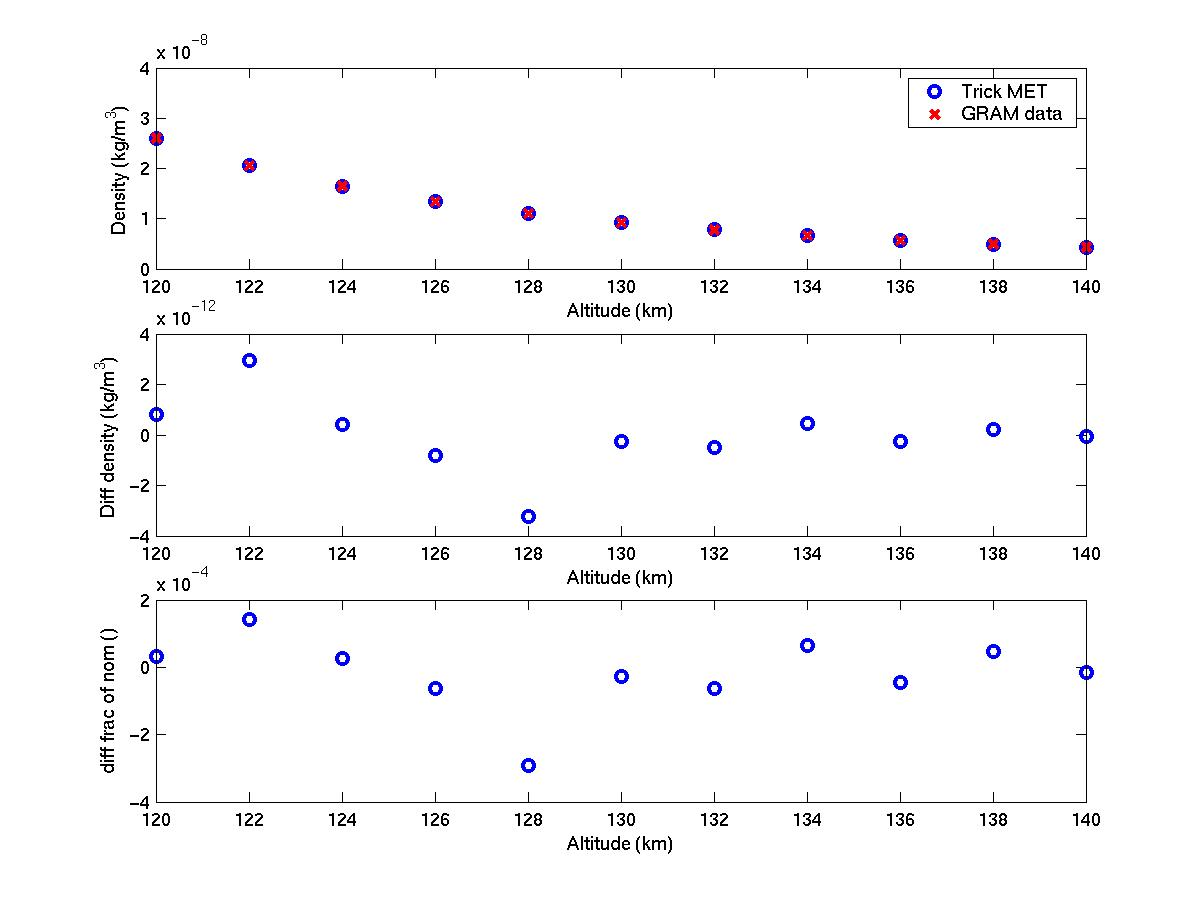
\includegraphics[height=80mm]{pics/MET_T01_density.jpg}
\caption{Density Comparison Between MET and Published GRAM Data}
\label{MET_dens_pub_comp}
\end{center}
\end{figure}

As Figure \ref{MET_dens_pub_comp} shows, the comparison between the MET model
and the GRAM outputs is excellent.  In the documentation, the density is
only given to four decimal places and this is why the comparison is only
accurate to a fraction of this fourth decimal place.

Figures \ref{MET_press_pub_comp} and \ref{MET_temp_pub_comp} show the results
of a comparison between the pressure and temperature output from the GRAM and
published results.

\begin{figure}[H]
\begin{center}
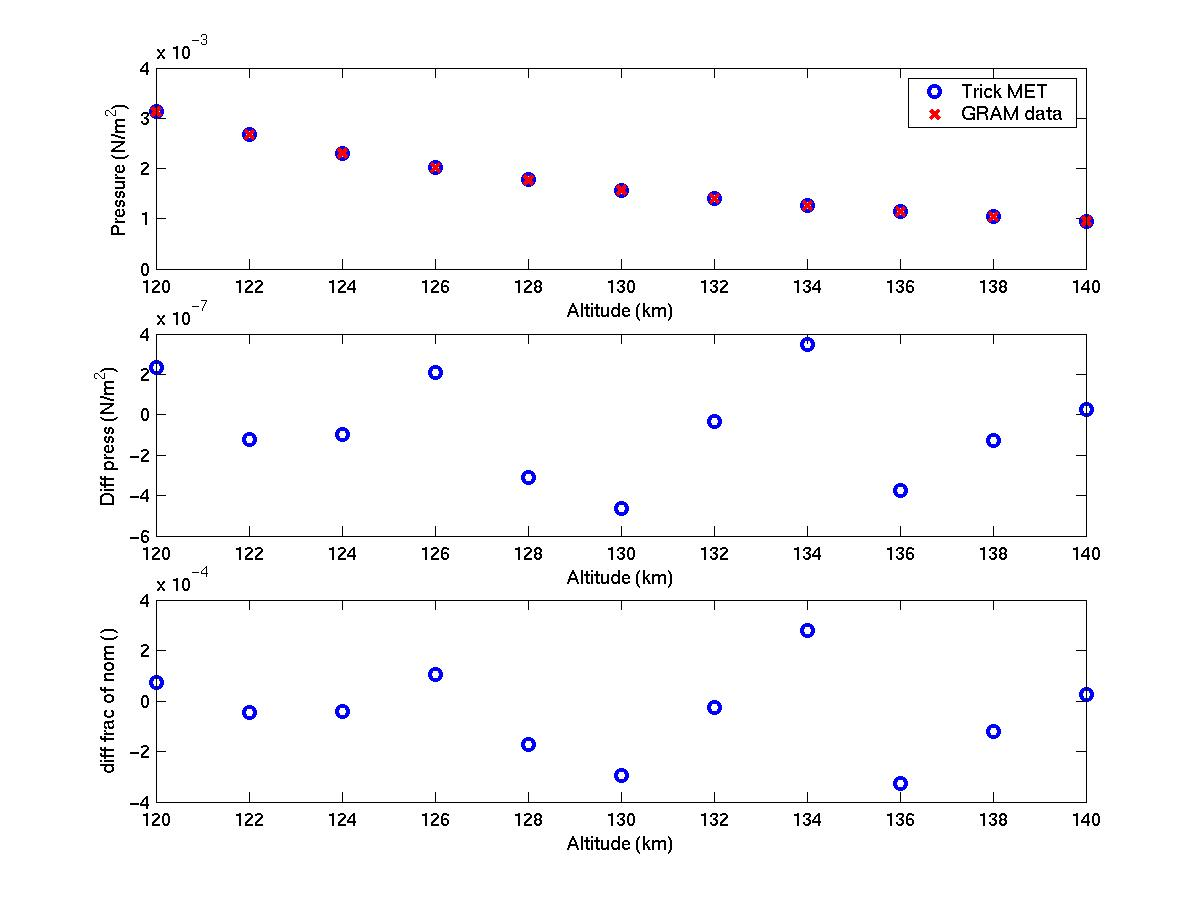
\includegraphics[height=80mm]{pics/MET_T01_pressure.jpg}
\caption{Pressure Comparison Between MET and Published GRAM Data}
\label{MET_press_pub_comp}
\end{center}
\end{figure}

\begin{figure}[H]
\begin{center}
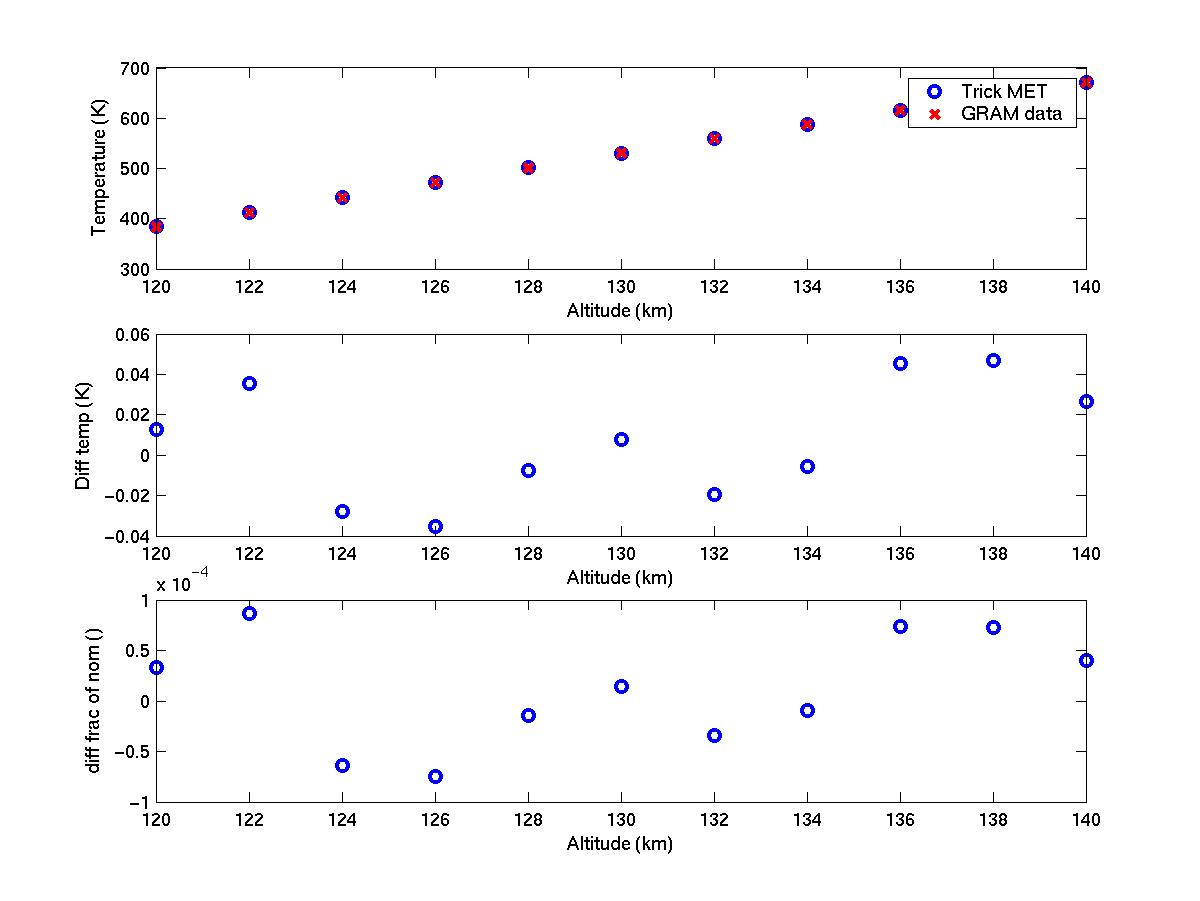
\includegraphics[height=80mm]{pics/MET_T01_temperature.jpg}
\caption{Temperature Comparison Between MET and Published GRAM Data}
\label{MET_temp_pub_comp}
\end{center}
\end{figure}

Both of these plots also exhibit the expected behavior.  In both cases,
the data was only available to 4 decimal places.
\end{description}

\test{MET Comparison with MSIS results}\label{test:met_MSIS}
\begin{description}
\item[Purpose:] \ \newline
SIM directory: SIM\_MET \newline
RUN directory: SET\_test/RUN\_T02\_MET\_VER

The purpose of this test is to compare the output of the Trick MET model
with the output from the MSIS model.

\item[Requirements:] \ \newline
By passing this test, the MET module partially satisfies
requirement~\ref{reqt:met_atmosphere}
\item[Procedure:]\ \newline
This test is designed to compare the density computed by the MET model
with results from the MSIS model.  The MSIS model is another atmosphere
model whose results are readily available although the results should
not compare with the MET model as accurately as the GRAM model does.

\item[Results:]\ \newline

Figure \ref{MET_MSIS_compare} shows a plot of a comparison between the density
output from the MET model and the density output from the MSIS model.

\begin{figure}[H]
\begin{center}
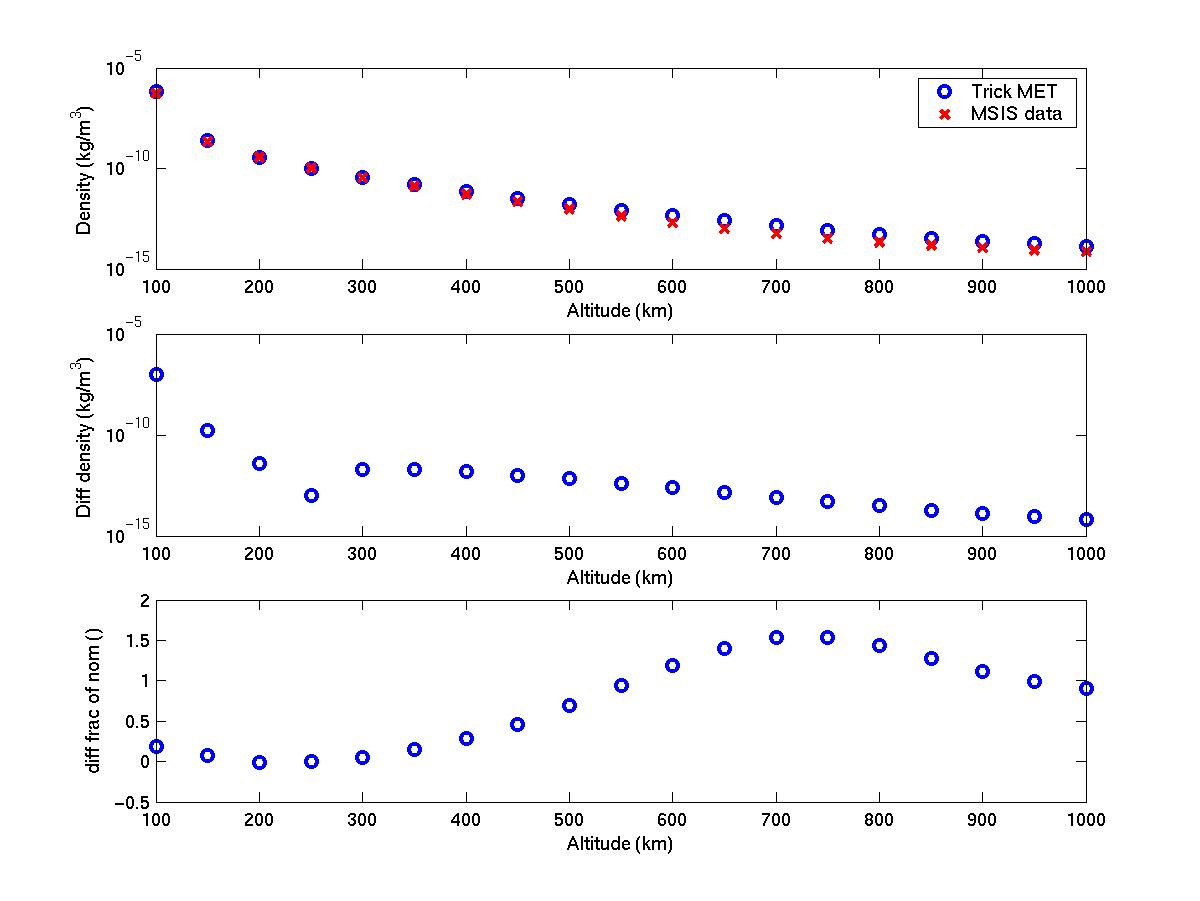
\includegraphics[height=80mm]{pics/MET_MSIS_T01_temperature.jpg}
\caption{Density Comparison Between MET and MSIS Data}
\label{MET_MSIS_compare}
\end{center}
\end{figure}

As this plot shows, the agreement between the MSIS data and the MET data is
not nearly as good as the agreement between MET and GRAM.  However, the MET
and MSIS model are both very consistent with each other throughout the range
of altitudes used.  And while they are occasionally off from each other by
as much as the MSIS density, this occurs when the value for the density is
extremely small.
\end{description}

\test{MET Comparison with Jacchia results}\label{test:met_JAC}
\begin{description}
\item[Purpose:] \ \newline
SIM directory: SIM\_MET \newline
RUN directory: SET\_test/RUN\_T01\_JAC\_COMP \newline
RUN directory: SET\_test/RUN\_T02\_JAC\_COMP

The purpose of this test is to compare the results of the MET model, the
Jacchia model, and the MSIS model to determine the consistency of the
MET model with respect to the other two and to determine if there is an
advantage to using the MET model over the Jacchia model.

\item[Requirements:] \ \newline
By passing this test, the MET module partially satisfies
requirement~\ref{reqt:met_atmosphere}
\item[Procedure:]\ \newline
This test is designed to compare the density computed
by the MET model with results from the Jacchia model.  The Jacchia model is
another atmosphere model available in Trick although it has not been verified.
The output from both models was compared with the output from the MSIS model
to determine whether or not there was a benefit to using the Jacchia model over
the MET model.
\item[Results:]\ \newline
Figure \ref{met_jac_global} shows a plot of a comparison between the MET and
MSIS models and the Jacchia and MSIS models.  This plot is designed to quantify
whether or not and how much of an advantage there exists in using one model
over the other.

\begin{figure}[H]
\begin{center}
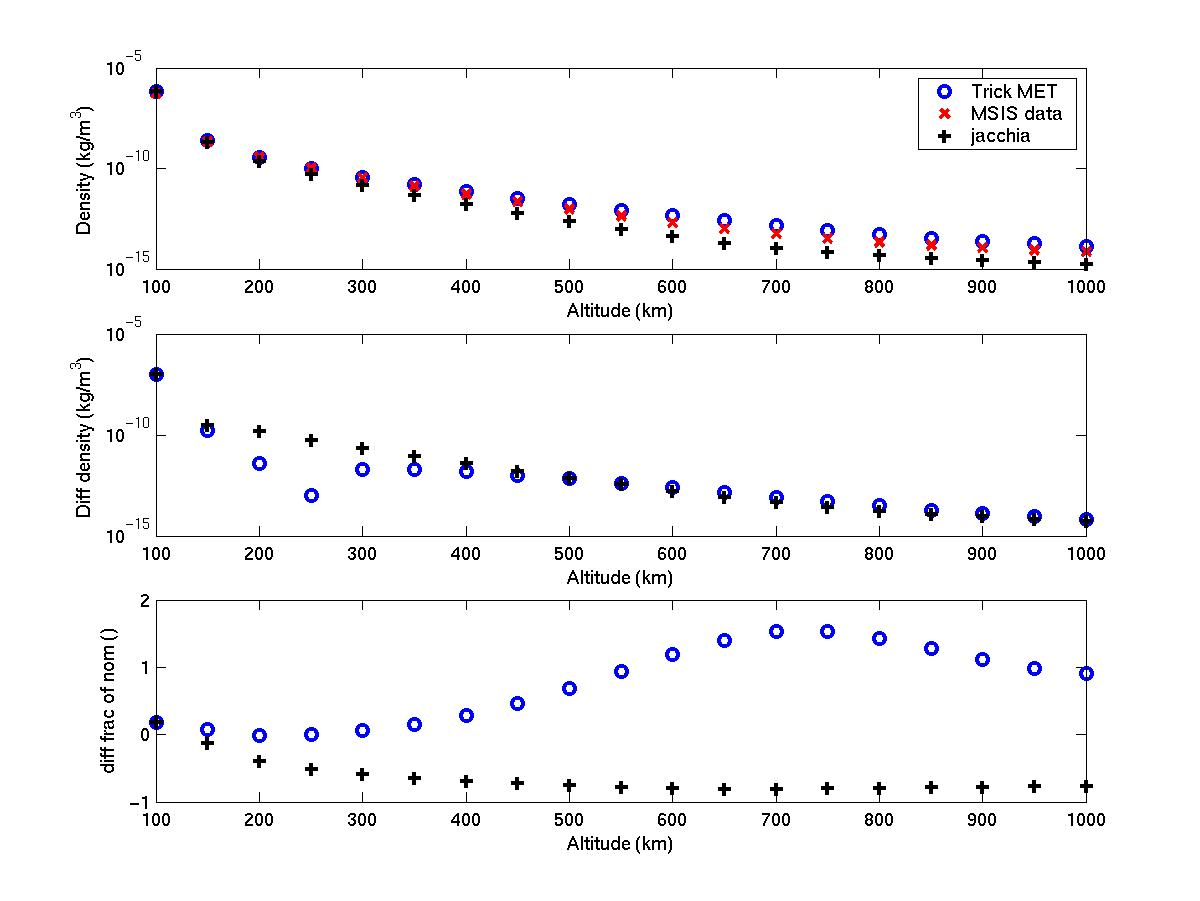
\includegraphics[height=80mm]{pics/MET_JAC_T01_temperature.jpg}
\caption{Density Comparison Between MET, Jacchia, and MSIS Data}
\label{met_jac_global}
\end{center}
\end{figure}

As this plot shows, the Jacchia model actual exhibits more agreement with the
MSIS model for the majority of the altitude range.  However, for the critical
range of altitudes where atmospheric drag is a factor for rendezvous analyses,
(0-500 km), the performance of the two models compared to the MSIS data.
Figure \ref{met_jac_critical} shows a comparison plot between the three models
for this critical range.

\begin{figure}[H]
\begin{center}
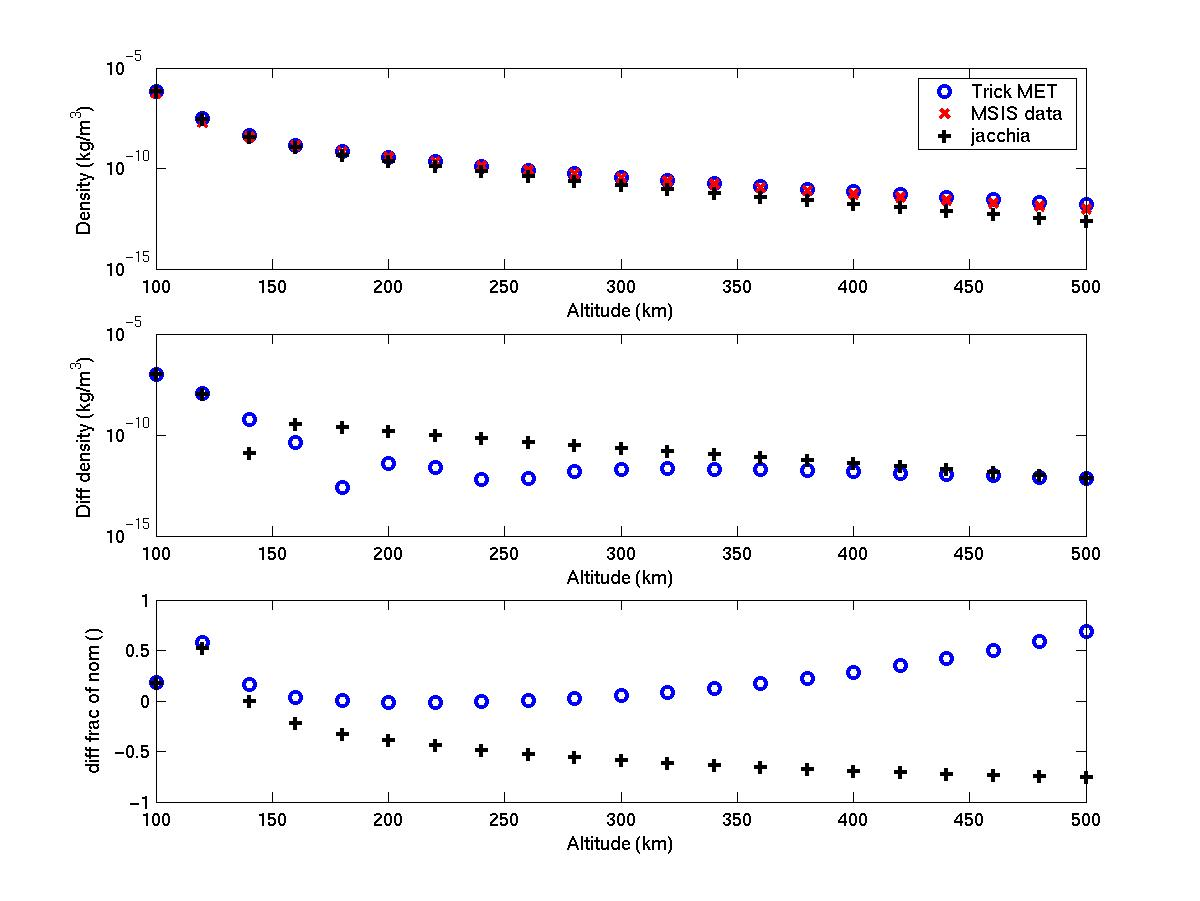
\includegraphics[height=80mm]{pics/MET_JAC_T02_temperature.jpg}
\caption{Density Comparison (100-500km) Between MET, Jacchia, and MSIS Data}
\label{met_jac_critical}
\end{center}
\end{figure}

As this plot shows, there is a slight advantage gained by using the MET model
instead of the Jacchia model for this range.  More importantly, it can be said
from these results that the agreement between Jacchia and MET is quite good when
the level of error of atmosphere estimation at these altitudes is taken into
account.  The added complexity of the Jacchia model and the increased overhead
required for its use certainly make the argument about why the MET model should
be used over the Jacchia model.  The MET model is much simpler to use in an
S\_define and relies on many fewer models and provides at least as good an
estimation of the Jacchia model and for the range of altitudes used for RPOC
work, it provides better agreement with MSIS.
\end{description}

\test{MET Comparison with FORTRAN GRAM results}\label{test:met_CML_GRAM}
\begin{description}
\item[Purpose:] \ \newline
SIM directory: SIM\_MET \newline
RUN directory: SET\_test/RUN\_T01\_GRAM\_MET \newline
RUN directory: SET\_test/RUN\_T02\_GRAM\_MET \newline
RUN directory: SET\_test/RUN\_T03\_GRAM\_MET

The purpose of this test is to compare the MET model with a more representative
set of data from the GRAM model.  There is a version of the GRAM model set up
to run in Trick available.  This model is FORTRAN code and has been used
for several projects and is considered to be an accurate model.  Furthermore, it
is very unlikely that MET and this model would both agree and not be
representative of the true MET model since they were programmed independently.

\item[Requirements:] \ \newline
By passing this test, the MET module partially satisfies
requirement~\ref{reqt:met_atmosphere}
\item[Procedure:]\ \newline
This test is designed to compare the output of the GRAM and MET model for a full
range of altitudes, latitudes, and longitudes.  Three test cases were run here
and the results are shown below.  The altitude was varied from 100 to 1500 km
above the surface of the ellipsoid.  The latitude was varied from -90 to 90
degrees.  The longitude was varied from -180 to 180 degrees.

\item[Results:]\ \newline
For each test, the density, pressure, and temperature were compared with each
other to determine the level of variation. Figures \ref{met_gram_alt_dens},
\ref{met_gram_alt_press}, and \ref{met_gram_alt_temp} show plots of the density,
pressure, and temperature variation as a function of the variation in altitude
used for the first test.

\begin{figure}[H]
\begin{center}
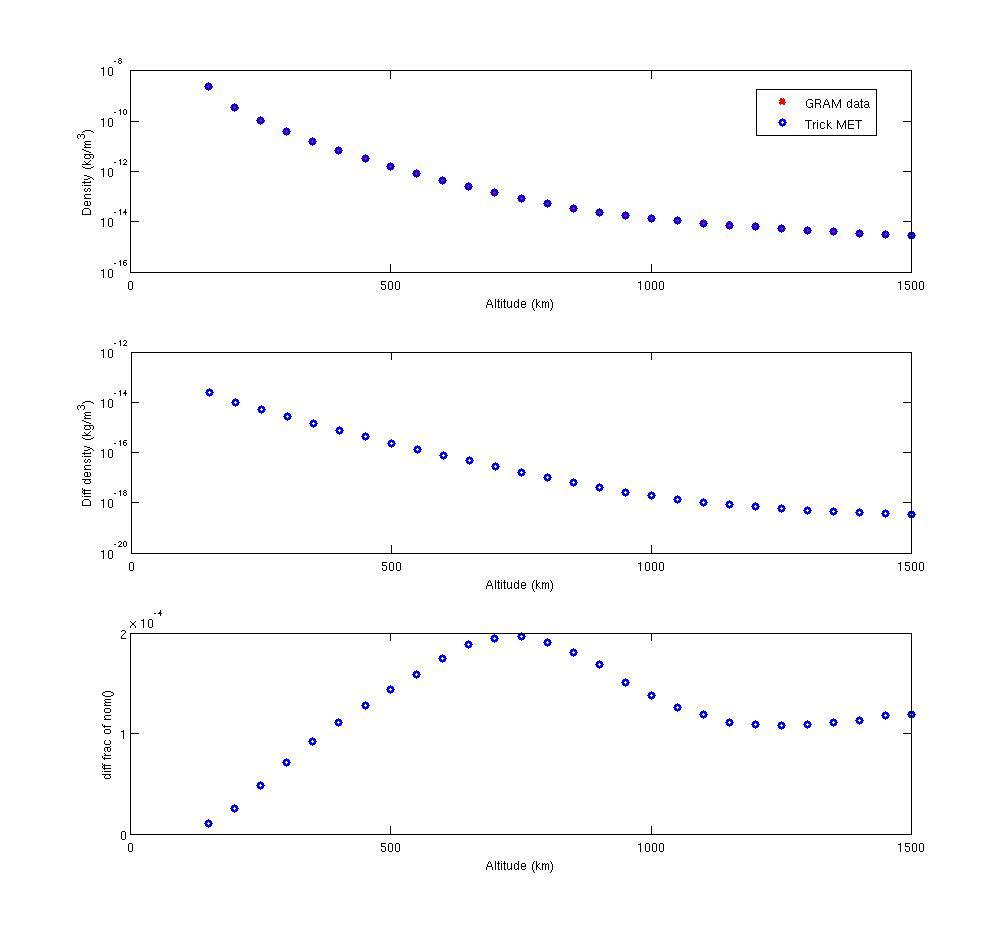
\includegraphics[height=80mm]{pics/MET_GRA_T01_density.jpg}
\caption{Density Comparison Between MET and GRAM for Altitude Variation}
\label{met_gram_alt_dens}
\end{center}
\end{figure}

\begin{figure}[H]
\begin{center}
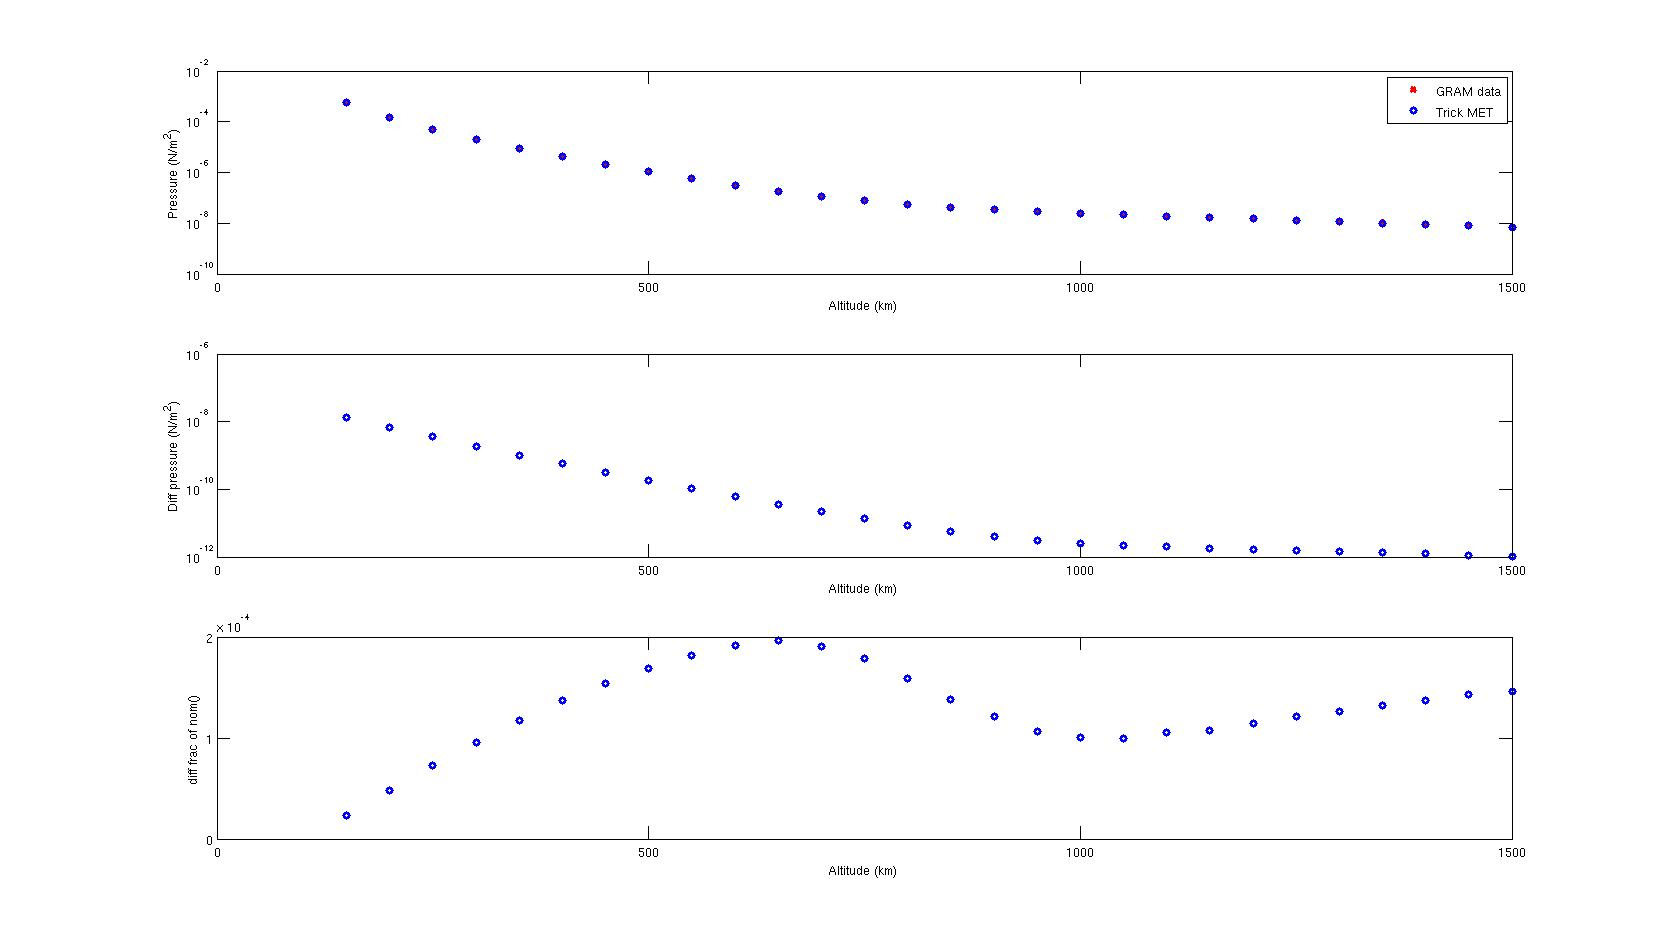
\includegraphics[height=80mm]{pics/MET_GRA_T01_pressure.jpg}
\caption{Pressure Comparison Between MET and GRAM for Altitude Variation}
\label{met_gram_alt_press}
\end{center}
\end{figure}

\begin{figure}[H]
\begin{center}
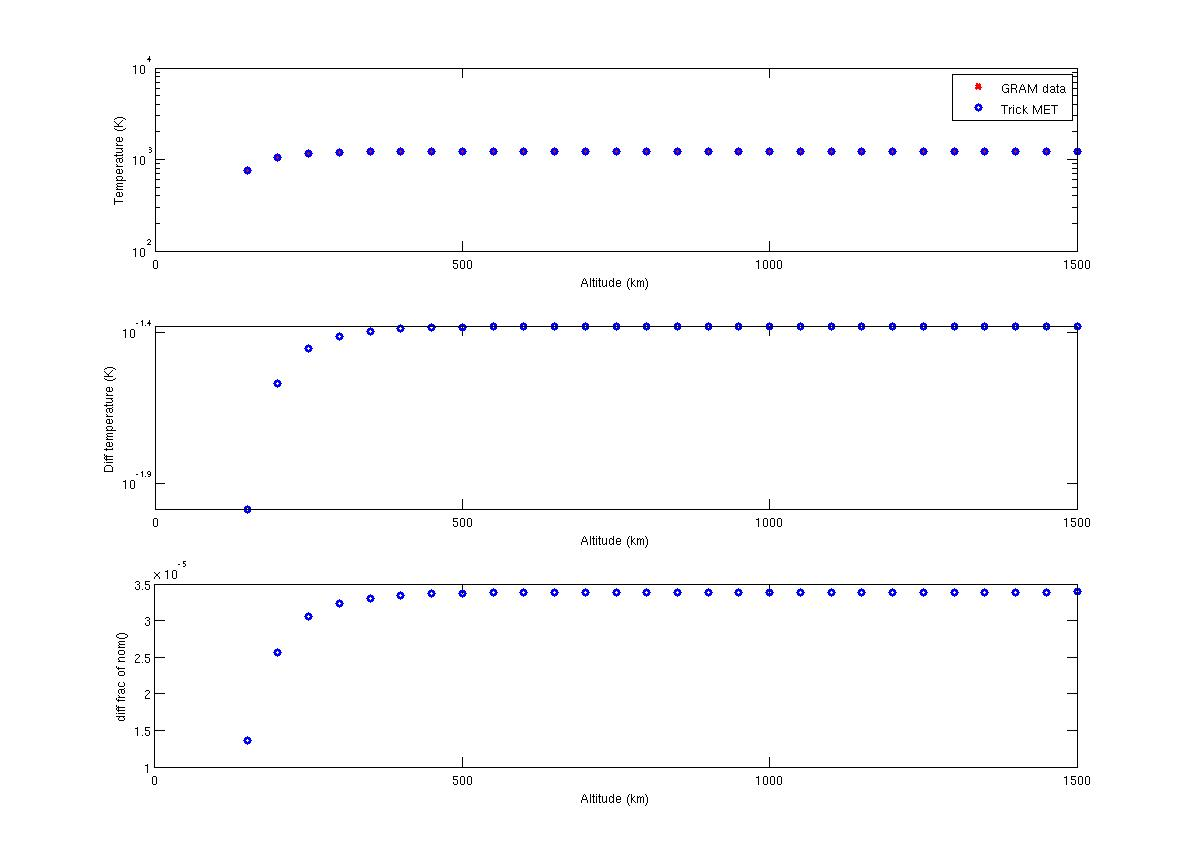
\includegraphics[height=80mm]{pics/MET_GRA_T01_temperature.jpg}
\caption{Temperature Comparison Between MET and GRAM for Altitude Variation}
\label{met_gram_alt_temp}
\end{center}
\end{figure}

As these plots show, for the altitude variation test, the results all agree to
approximately 4 significant digits.  Figures \ref{met_gram_lat_dens},
\ref{met_gram_lat_press}, and \ref{met_gram_lat_temp} show the results for the
test that varied the latitude of the spacecraft.

\begin{figure}[H]
\begin{center}
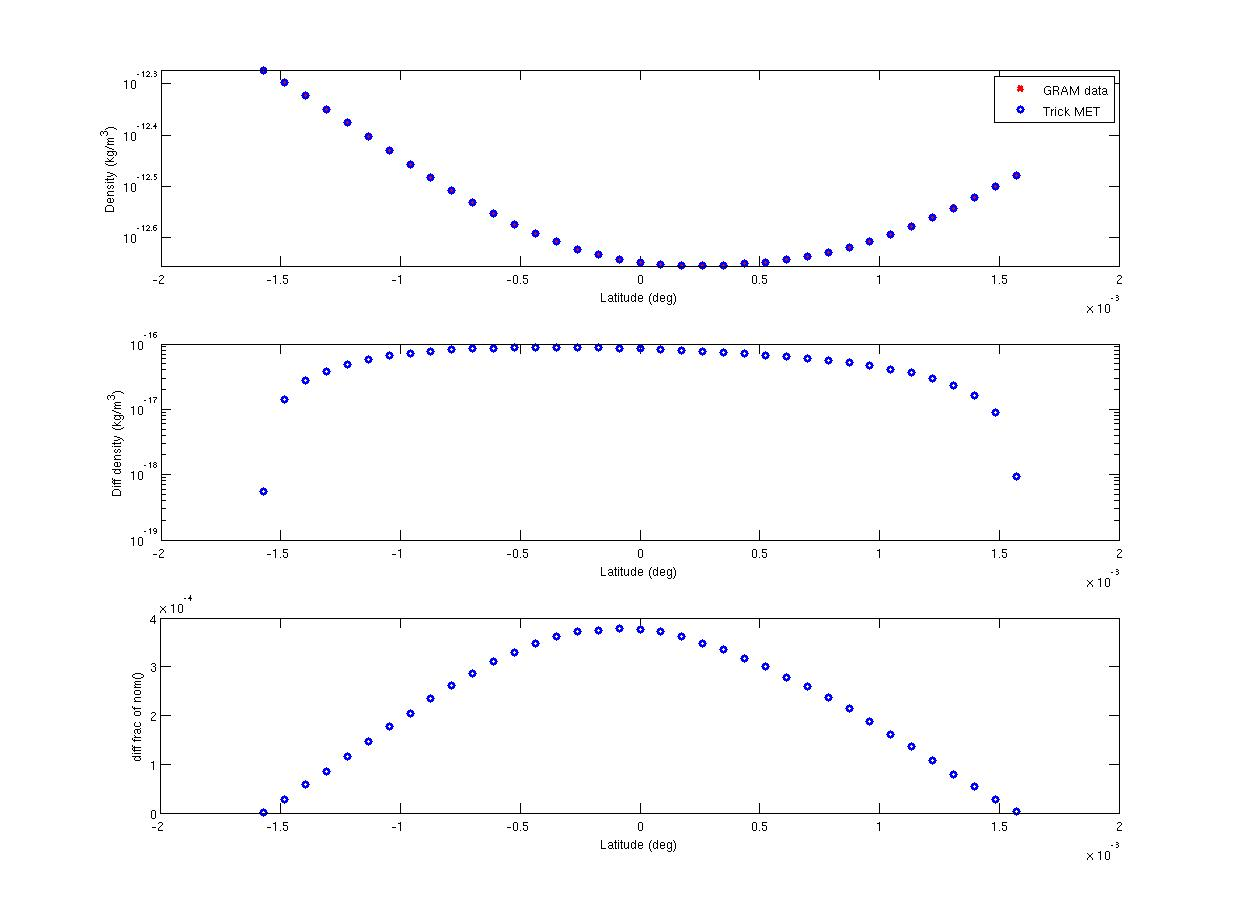
\includegraphics[height=80mm]{pics/MET_GRA_T02_density.jpg}
\caption{Density Comparison Between MET and GRAM for Latitude Variation}
\label{met_gram_lat_dens}
\end{center}
\end{figure}

\begin{figure}[H]
\begin{center}
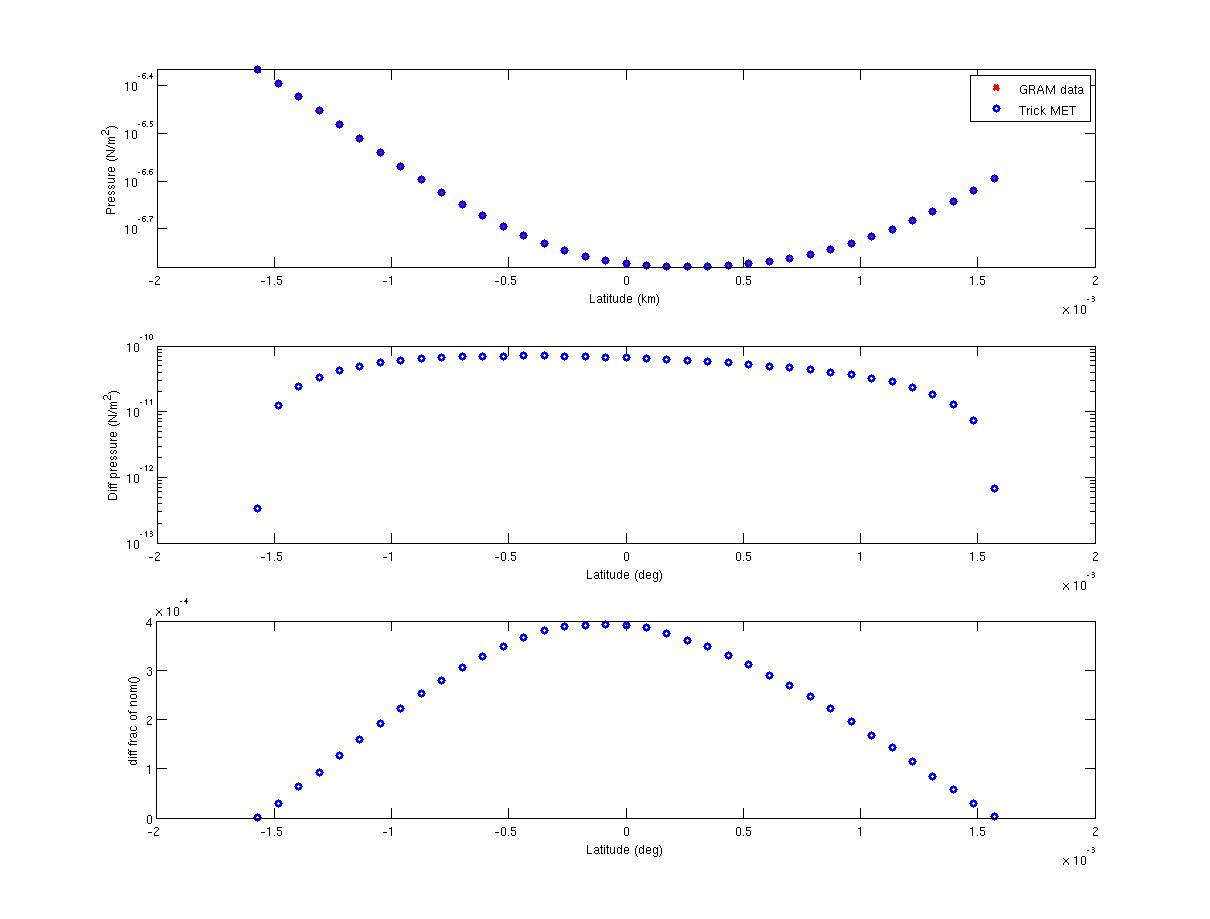
\includegraphics[height=80mm]{pics/MET_GRA_T02_pressure.jpg}
\caption{Pressure Comparison Between MET and GRAM for Latitude Variation}
\label{met_gram_lat_press}
\end{center}
\end{figure}

\begin{figure}[H]
\begin{center}
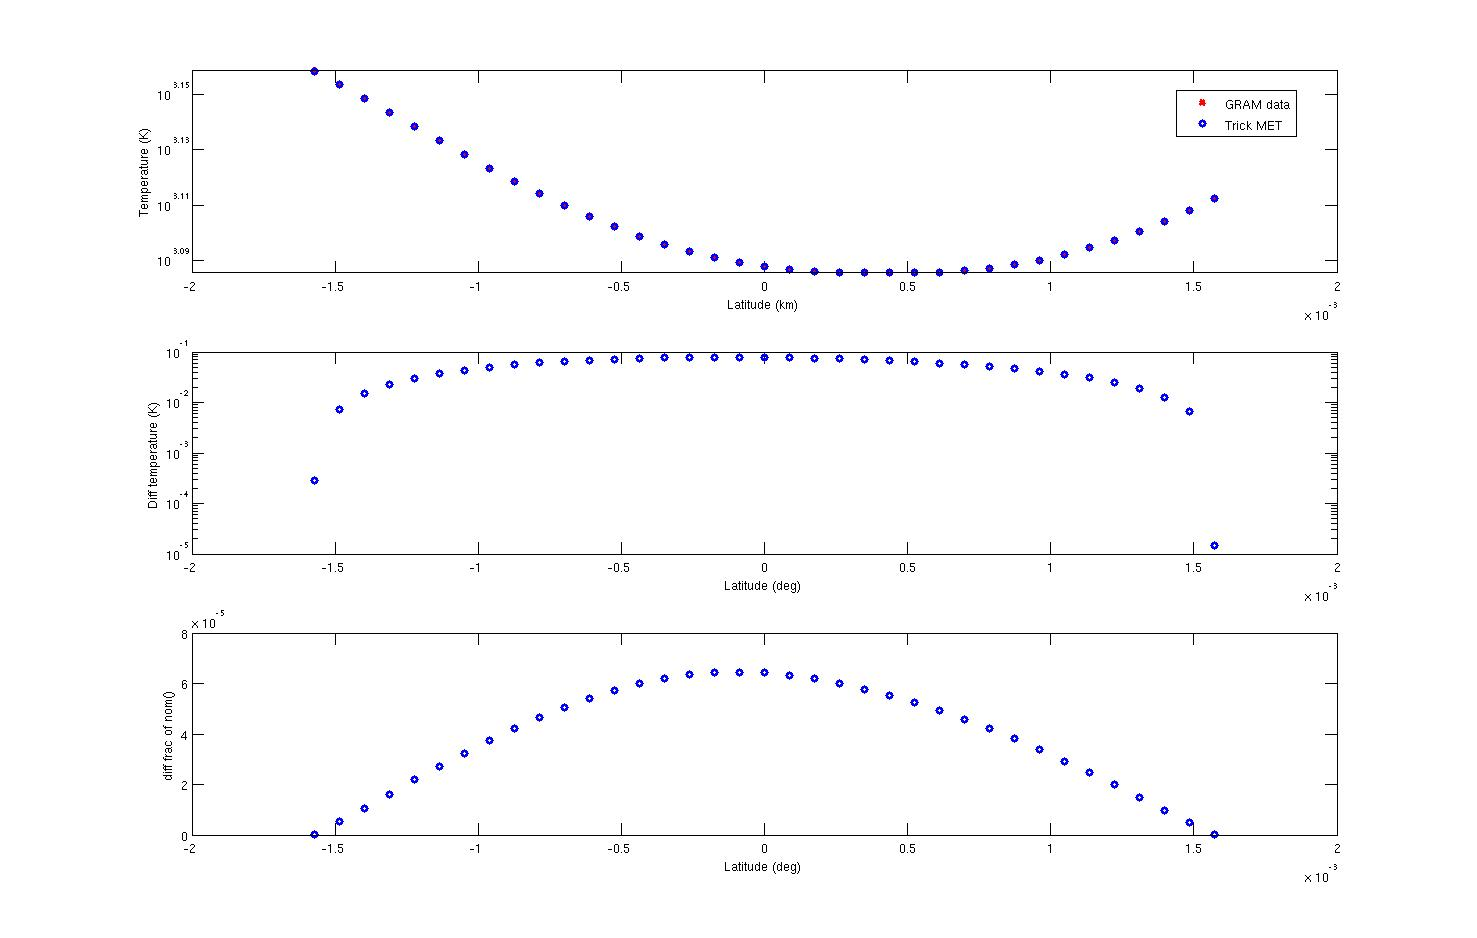
\includegraphics[height=80mm]{pics/MET_GRA_T02_temperature.jpg}
\caption{Temperature Comparison Between MET and GRAM for Latitude Variation}
\label{met_gram_lat_temp}
\end{center}
\end{figure}

As these plots show, the results of the test on spacecraft latitude were also
consistent to approximately 4 significant digits.  In this case, the reference
altitude was chosen as 650 meters because that altitude had a higher general
level of error in the first set of plots.  Figures \ref{met_gram_lon_dens},
\ref{met_gram_lon_press}, and \ref{met_gram_lon_temp} show the results for the
test that varied the longitude of the spacecraft.

\begin{figure}[H]
\begin{center}
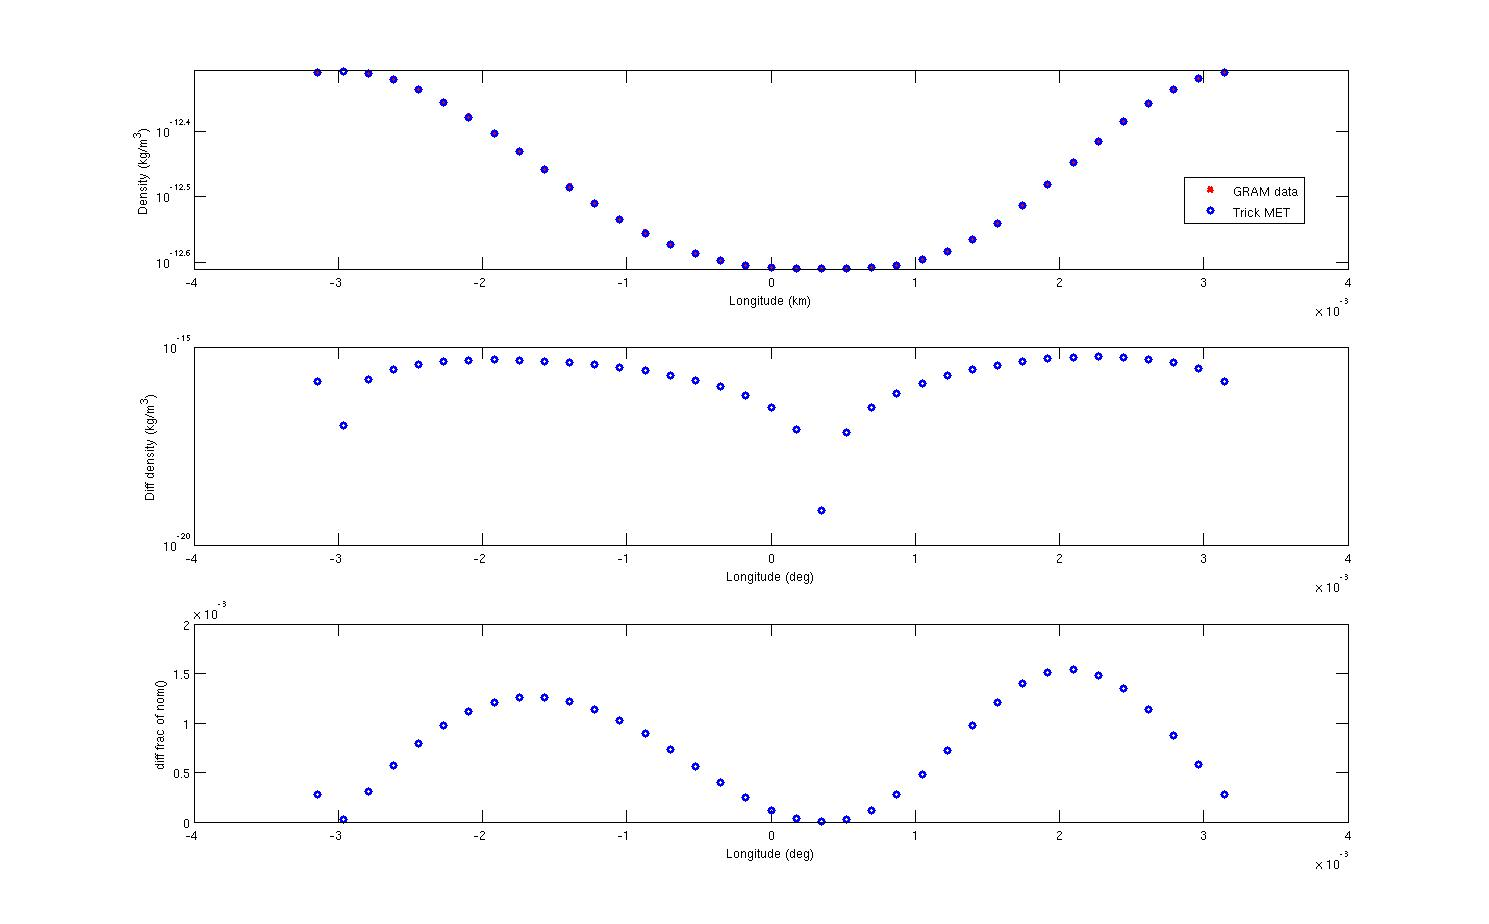
\includegraphics[height=80mm]{pics/MET_GRA_T03_density.jpg}
\caption{Density Comparison Between MET and GRAM for Longitude Variation}
\label{met_gram_lon_dens}
\end{center}
\end{figure}

\begin{figure}[H]
\begin{center}
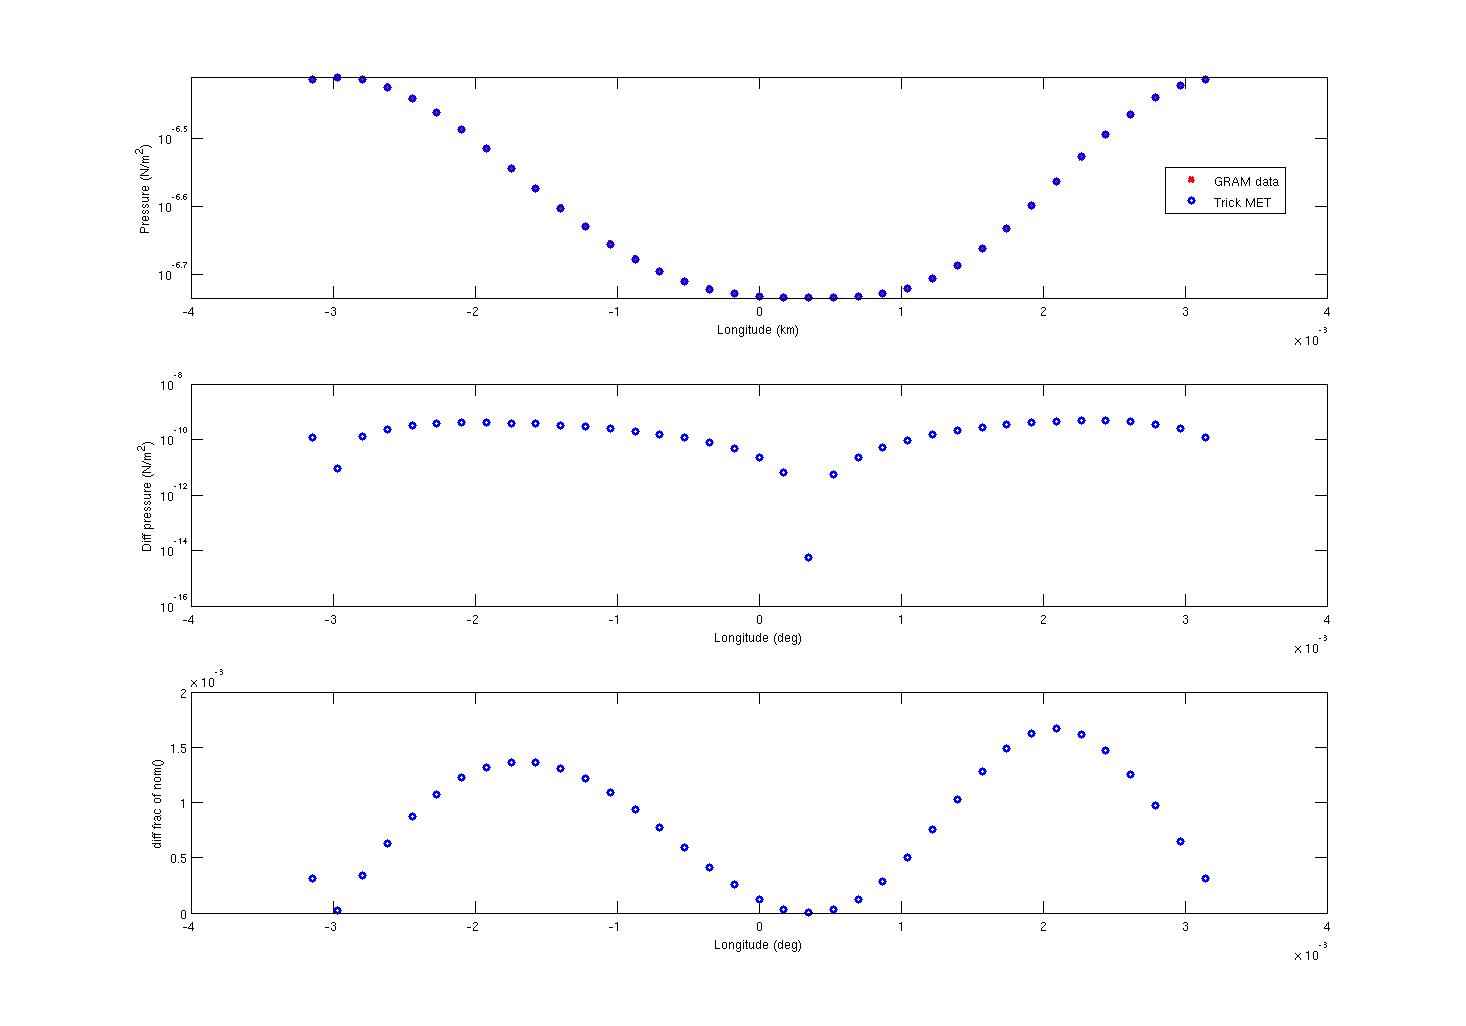
\includegraphics[height=80mm]{pics/MET_GRA_T03_pressure.jpg}
\caption{Pressure Comparison Between MET and GRAM for Longitude Variation}
\label{met_gram_lon_press}
\end{center}
\end{figure}

\begin{figure}[H]
\begin{center}
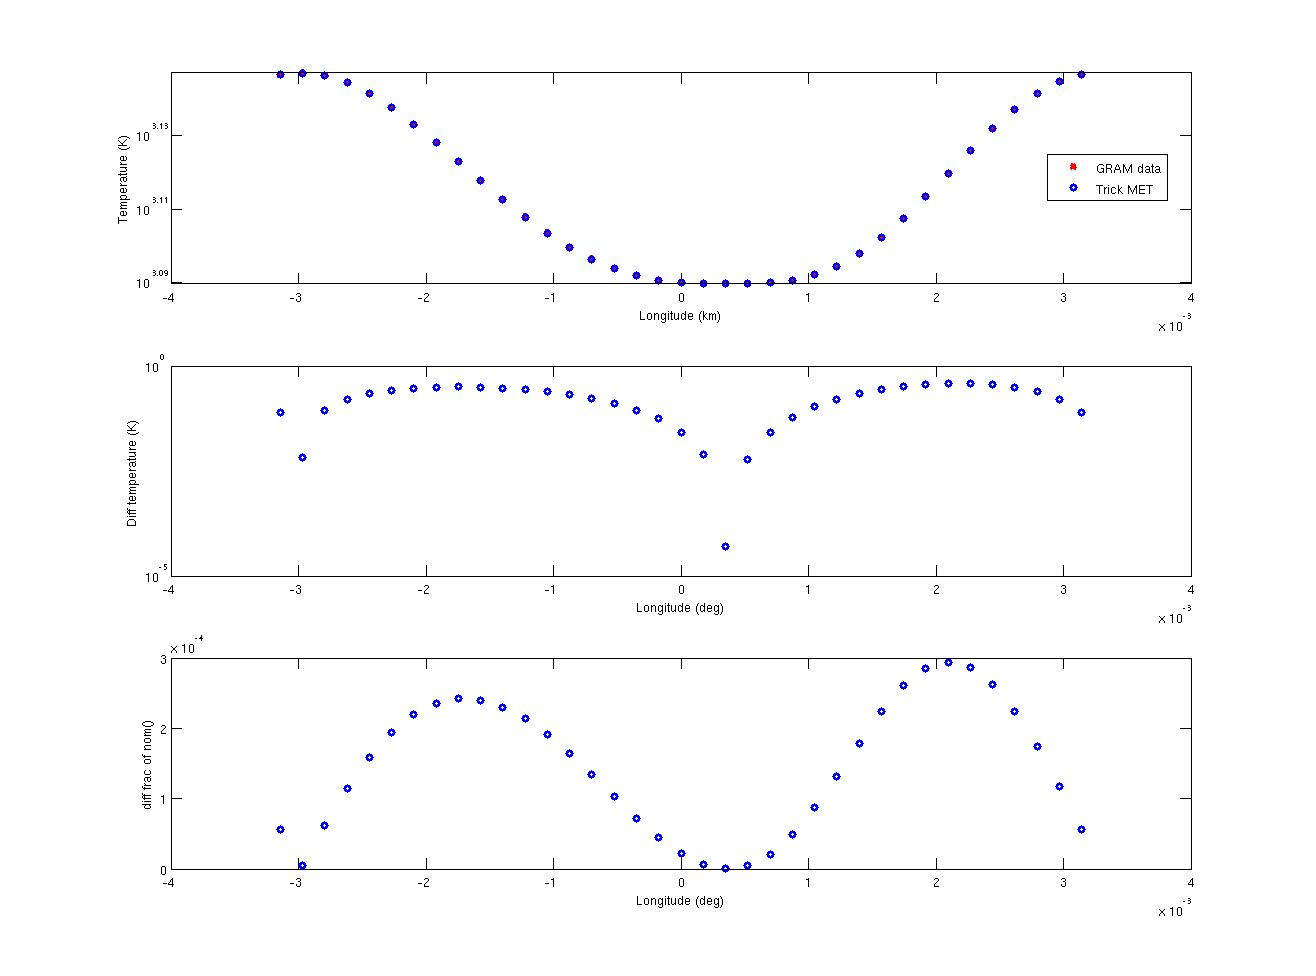
\includegraphics[height=80mm]{pics/MET_GRA_T03_temperature.jpg}
\caption{Temperature Comparison Between MET and GRAM for Longitude Variation}
\label{met_gram_lon_temp}
\end{center}
\end{figure}

From all of these plots, it is apparent that the MET model used in Trick matches
up with the GRAM model found in the (GRAM/MET 99) to three to four digits.
Because the atmosphere parameters are never known to this level of precision,
this level of agreement is considered more than accurate for the model.

Additionally, there is a known discrepancy between the MET mode used
for JEOD and the GRAM model used here for comparison. As stated in the
JEOD 1.52 documentation for this model \cite{atmosphere_15}, it was discovered
that there were small discontinuities in the output of the GRAM model, occuring
at each minute. This was because the GRAM model used was constructed to ignore
the ``seconds" parameter from its inputted calendar date. Thus, the source
code for the JEOD implementation of MET, which also originally had this
peculiarity, was changed to include the second parameter into the calculation.
Prior to this change, the models matched to six digits; they now only match
to 3-4 digits, but because this implementation appears to be more consistent
and stable, it was decided that this level of error was acceptable.
\end{description}


\section{Metrics}
\subsection{Code Metrics}

Table~\ref{tab:coarse_metrics} presents coarse metrics on the
source files that comprise the model.

\input{coarse_metrics}

Table~\ref{tab:metrix_metrics} presents the extended cyclomatic
complexity
(ECC) of the methods defined in the model.
\input{metrix_metrics}


\section{Requirements Traceability}\label{sec:traceability}

\begin{longtable}[c]{||p{3in}|p{3in}|}
\caption{Requirements Traceability} \\[6pt]
\hline
{\bf Requirement} & {\bf Inspection and Testing} \\
\hline \hline
\endfirsthead
\hline
\endfoot
\caption[]{Requirements Traceability (continued)} \\[6pt]
\hline
{\bf Requirement} & {\bf Inspection and Testing} \\
\hline \hline
\endhead

\ref{reqt:toplevel} - Top-level Requirements &
  Inspection~\ref{inspect:TLI} \\
  \hline

\ref{reqt:met_atmosphere} - MET Atmosphere &
   Test~\ref{test:met_GRAM_99} \\
   &Test~\ref{test:met_MSIS} \\
   &Test~\ref{test:met_JAC} \\
   &Test~\ref{test:met_CML_GRAM} \\

   \hline

 \ref{reqt:atmos_extension} - Atmosphere Extensibility &
   Inspection~\ref{inspect:extension} \\
 \hline

 \ref{reqt:atmos_wind} - Wind Model &
   Inspection~\ref{inspect:wind} \\

 \hline

\end{longtable}


%%% or for a document with multiple parts make as many copies of Chapters.tex
%%% as you have parts and use this format
%\hyperdef{part}{part1}{\part{Part 1 Title}}\label{pt1:title}
%\include{atmosphereChapters1}
%\hyperdef{part}{part2}{\part{Part 2 Title}}\label{pt2:title}
%\include{atmosphereChapters2}
%%% etc.

%%%%%%%%%%%%%%%%%%%%%%%%%%%%%%%%%%%%%%%%%%%%%%%%%%%%%%%%%%%%%%%%%%%%%%%%%
% Bibliography
%%%%%%%%%%%%%%%%%%%%%%%%%%%%%%%%%%%%%%%%%%%%%%%%%%%%%%%%%%%%%%%%%%%%%%%%%
\newpage
\pdfbookmark{Bibliography}{bibliography}
\bibliography{dynenv,atmosphere}
\bibliographystyle{plain}

%\pagebreak
%\appendix

\end{document}
